%\documentclass[fleqn,usenatbib]{aa}
%DIF LATEXDIFF DIFFERENCE FILE
%DIF DEL forestflow_cwr_fordiff.tex   Thu Jul 25 12:39:36 2024
%DIF ADD forestflow_after_cwr.tex     Thu Jul 25 12:12:44 2024
\documentclass{aa}

\usepackage{newtxtext,newtxmath}
\usepackage[T1]{fontenc}

% \DeclareRobustCommand{\VAN}[3]{#2}
% \let\VANthebibliography\thebibliography
% \def\thebibliography{\DeclareRobustCommand{\VAN}[3]{##3}\VANthebibliography}
\usepackage{color}
\usepackage{natbib,twoopt}
\usepackage[hyphenbreaks]{breakurl}
\usepackage[breaklinks]{hyperref}

\usepackage{graphicx}
\usepackage{upgreek}

% \usepackage{txfonts}
% \usepackage{amsmath}
\usepackage{xspace}
% \usepackage[table]{xcolor}
% \usepackage[normalem]{ulem}


\bibpunct{(}{)}{;}{a}{}{,}
\definecolor{cobalt}{rgb}{0.06, 0.2, 0.65}
\hypersetup{
  colorlinks,
  citecolor=cobalt,
  linkcolor=[rgb]{0.8, 0.2, 1.0},
  urlcolor=cobalt,
}



%%%%%%%%%%%%%%%%%%%%%%%%%%%%%%%%%%%%%%%%%%%%%%%%%%

\newcommand{\lya}{Lyman-$\alpha$\xspace}
\newcommand{\lyaf}{Lyman-$\alpha$ forest\xspace}
\newcommand{\pcross}{$P_{\times}$\xspace}
\newcommand{\poned}{\ensuremath{P_{\rm 1D}}\xspace}
\newcommand{\xithreed}{\ensuremath{\xi_{\rm 3D}}\xspace}
\newcommand{\pthreed}{\ensuremath{P_{\rm 3D}}\xspace}

\newcommand{\forestflow}{\textsc{forestflow}\xspace}

\newcommand{\lacehc}{\textsc{training}\xspace}
\newcommand{\simseed}{\textsc{seed}\xspace}
\newcommand{\simigm}{\textsc{reionisation}\xspace}
\newcommand{\simcurved}{\textsc{curved}\xspace}
\newcommand{\simh}{\textsc{growth}\xspace}
\newcommand{\simnu}{\textsc{neutrinos}\xspace}
\newcommand{\simns}{\textsc{running}\xspace}
\newcommand{\simcentral}{\textsc{central}\xspace}

\newcommand{\mflux}{\ensuremath{\bar{F}}\xspace}
\newcommand{\iMpc}{\ensuremath{\,\mathrm{Mpc}^{-1}}}
\newcommand{\hMpc}{h^{-1}\,\mathrm{Mpc}}

% \defcitealias{Pedersen2021}{P21}

\newcommand{\jch}[1]{ {\color{orange} [JCH: #1]}}
\newcommand{\lc}[1]{ {\color{magenta} #1}}
\newcommand{\ml}[1]{ {\color{green} [ML: #1]}}
\newcommand{\afr}[1]{ {\color{red} [AFR: #1]}}




%%%%%%%%%%%%%%%%%%%%%%%%%%%%%%%%%%%%%%%%%%%%%%%%%%

%%%%%%%%%%%%%%%%%%% TITLE PAGE %%%%%%%%%%%%%%%%%%%
%DIF PREAMBLE EXTENSION ADDED BY LATEXDIFF
%DIF UNDERLINE PREAMBLE %DIF PREAMBLE
\RequirePackage[normalem]{ulem} %DIF PREAMBLE
\RequirePackage{color}\definecolor{RED}{rgb}{1,0,0}\definecolor{BLUE}{rgb}{0,0,1} %DIF PREAMBLE
\providecommand{\DIFaddtex}[1]{{\protect\color{blue}\uwave{#1}}} %DIF PREAMBLE
\providecommand{\DIFdeltex}[1]{{\protect\color{red}\sout{#1}}}                      %DIF PREAMBLE
%DIF SAFE PREAMBLE %DIF PREAMBLE
\providecommand{\DIFaddbegin}{} %DIF PREAMBLE
\providecommand{\DIFaddend}{} %DIF PREAMBLE
\providecommand{\DIFdelbegin}{} %DIF PREAMBLE
\providecommand{\DIFdelend}{} %DIF PREAMBLE
\providecommand{\DIFmodbegin}{} %DIF PREAMBLE
\providecommand{\DIFmodend}{} %DIF PREAMBLE
%DIF FLOATSAFE PREAMBLE %DIF PREAMBLE
\providecommand{\DIFaddFL}[1]{\DIFadd{#1}} %DIF PREAMBLE
\providecommand{\DIFdelFL}[1]{\DIFdel{#1}} %DIF PREAMBLE
\providecommand{\DIFaddbeginFL}{} %DIF PREAMBLE
\providecommand{\DIFaddendFL}{} %DIF PREAMBLE
\providecommand{\DIFdelbeginFL}{} %DIF PREAMBLE
\providecommand{\DIFdelendFL}{} %DIF PREAMBLE
%DIF HYPERREF PREAMBLE %DIF PREAMBLE
\providecommand{\DIFadd}[1]{\texorpdfstring{\DIFaddtex{#1}}{#1}} %DIF PREAMBLE
\providecommand{\DIFdel}[1]{\texorpdfstring{\DIFdeltex{#1}}{}} %DIF PREAMBLE
\newcommand{\DIFscaledelfig}{0.5}
%DIF HIGHLIGHTGRAPHICS PREAMBLE %DIF PREAMBLE
\RequirePackage{settobox} %DIF PREAMBLE
\RequirePackage{letltxmacro} %DIF PREAMBLE
\newsavebox{\DIFdelgraphicsbox} %DIF PREAMBLE
\newlength{\DIFdelgraphicswidth} %DIF PREAMBLE
\newlength{\DIFdelgraphicsheight} %DIF PREAMBLE
% store original definition of \includegraphics %DIF PREAMBLE
\LetLtxMacro{\DIFOincludegraphics}{\includegraphics} %DIF PREAMBLE
\newcommand{\DIFaddincludegraphics}[2][]{{\color{blue}\fbox{\DIFOincludegraphics[#1]{#2}}}} %DIF PREAMBLE
\newcommand{\DIFdelincludegraphics}[2][]{% %DIF PREAMBLE
\sbox{\DIFdelgraphicsbox}{\DIFOincludegraphics[#1]{#2}}% %DIF PREAMBLE
\settoboxwidth{\DIFdelgraphicswidth}{\DIFdelgraphicsbox} %DIF PREAMBLE
\settoboxtotalheight{\DIFdelgraphicsheight}{\DIFdelgraphicsbox} %DIF PREAMBLE
\scalebox{\DIFscaledelfig}{% %DIF PREAMBLE
\parbox[b]{\DIFdelgraphicswidth}{\usebox{\DIFdelgraphicsbox}\\[-\baselineskip] \rule{\DIFdelgraphicswidth}{0em}}\llap{\resizebox{\DIFdelgraphicswidth}{\DIFdelgraphicsheight}{% %DIF PREAMBLE
\setlength{\unitlength}{\DIFdelgraphicswidth}% %DIF PREAMBLE
\begin{picture}(1,1)% %DIF PREAMBLE
\thicklines\linethickness{2pt} %DIF PREAMBLE
{\color[rgb]{1,0,0}\put(0,0){\framebox(1,1){}}}% %DIF PREAMBLE
{\color[rgb]{1,0,0}\put(0,0){\line( 1,1){1}}}% %DIF PREAMBLE
{\color[rgb]{1,0,0}\put(0,1){\line(1,-1){1}}}% %DIF PREAMBLE
\end{picture}% %DIF PREAMBLE
}\hspace*{3pt}}} %DIF PREAMBLE
} %DIF PREAMBLE
\LetLtxMacro{\DIFOaddbegin}{\DIFaddbegin} %DIF PREAMBLE
\LetLtxMacro{\DIFOaddend}{\DIFaddend} %DIF PREAMBLE
\LetLtxMacro{\DIFOdelbegin}{\DIFdelbegin} %DIF PREAMBLE
\LetLtxMacro{\DIFOdelend}{\DIFdelend} %DIF PREAMBLE
\DeclareRobustCommand{\DIFaddbegin}{\DIFOaddbegin \let\includegraphics\DIFaddincludegraphics} %DIF PREAMBLE
\DeclareRobustCommand{\DIFaddend}{\DIFOaddend \let\includegraphics\DIFOincludegraphics} %DIF PREAMBLE
\DeclareRobustCommand{\DIFdelbegin}{\DIFOdelbegin \let\includegraphics\DIFdelincludegraphics} %DIF PREAMBLE
\DeclareRobustCommand{\DIFdelend}{\DIFOaddend \let\includegraphics\DIFOincludegraphics} %DIF PREAMBLE
\LetLtxMacro{\DIFOaddbeginFL}{\DIFaddbeginFL} %DIF PREAMBLE
\LetLtxMacro{\DIFOaddendFL}{\DIFaddendFL} %DIF PREAMBLE
\LetLtxMacro{\DIFOdelbeginFL}{\DIFdelbeginFL} %DIF PREAMBLE
\LetLtxMacro{\DIFOdelendFL}{\DIFdelendFL} %DIF PREAMBLE
\DeclareRobustCommand{\DIFaddbeginFL}{\DIFOaddbeginFL \let\includegraphics\DIFaddincludegraphics} %DIF PREAMBLE
\DeclareRobustCommand{\DIFaddendFL}{\DIFOaddendFL \let\includegraphics\DIFOincludegraphics} %DIF PREAMBLE
\DeclareRobustCommand{\DIFdelbeginFL}{\DIFOdelbeginFL \let\includegraphics\DIFdelincludegraphics} %DIF PREAMBLE
\DeclareRobustCommand{\DIFdelendFL}{\DIFOaddendFL \let\includegraphics\DIFOincludegraphics} %DIF PREAMBLE
%DIF LISTINGS PREAMBLE %DIF PREAMBLE
\RequirePackage{listings} %DIF PREAMBLE
\RequirePackage{color} %DIF PREAMBLE
\lstdefinelanguage{DIFcode}{ %DIF PREAMBLE
%DIF DIFCODE_UNDERLINE %DIF PREAMBLE
  moredelim=[il][\color{red}\sout]{\%DIF\ <\ }, %DIF PREAMBLE
  moredelim=[il][\color{blue}\uwave]{\%DIF\ >\ } %DIF PREAMBLE
} %DIF PREAMBLE
\lstdefinestyle{DIFverbatimstyle}{ %DIF PREAMBLE
	language=DIFcode, %DIF PREAMBLE
	basicstyle=\ttfamily, %DIF PREAMBLE
	columns=fullflexible, %DIF PREAMBLE
	keepspaces=true %DIF PREAMBLE
} %DIF PREAMBLE
\lstnewenvironment{DIFverbatim}{\lstset{style=DIFverbatimstyle}}{} %DIF PREAMBLE
\lstnewenvironment{DIFverbatim*}{\lstset{style=DIFverbatimstyle,showspaces=true}}{} %DIF PREAMBLE
%DIF END PREAMBLE EXTENSION ADDED BY LATEXDIFF

\begin{document}


\title{ForestFlow: cosmological emulation of Lyman-$\alpha$ forest clustering from linear to nonlinear scales}
\titlerunning{ForestFlow: emulating Lyman-$\alpha$ forest clustering}

\author{
J.~Chaves-Montero\inst{1}\thanks{jchaves@ifae.es}
\and
L.~Cabayol-Garcia\inst{1,2}\thanks{lcabayol@pic.es}
\and
M.~Lokken\inst{1}
\and
A.~Font-Ribera\inst{1}\thanks{afont@ifae.es}
\and
others
}

\institute{
Institut de F\'{\i}sica d'Altes Energies (IFAE), The Barcelona Institute of Science and Technology, 08193 Bellaterra (Barcelona), Spain
\and
Port d'Informaci\'{o} Cient\'{i}fica, Campus UAB, C. Albareda s/n, 08193 Bellaterra (Barcelona), Spain
}


\date{Received 2024; accepted XXX}

\abstract{
    On large scales, measurements of the Lyman-$\alpha$ forest offer insights into the expansion history of the Universe, while on small scales, these impose strict constraints on the growth history, the nature of dark matter, and the sum of neutrino masses. This work introduces \textsc{forestflow}, a cosmological emulator designed to bridge the gap between large- and small-scale analyses. Using conditional normalizing flows, \textsc{forestflow} emulates the 2 Lyman-$\alpha$ linear biases ($b_\delta$ and $b_\eta$) and 6 parameters describing small-scale deviations of the three-dimensional flux power spectrum ($P_\mathrm{3D}$) from linear theory. These 8 parameters are modeled as a function of cosmology --- the small-scale amplitude and slope of the linear power spectrum ---- and the physics of the intergalactic medium. Thus, in combination with a Boltzmann solver, \textsc{forestflow} can predict $P_\mathrm{3D}$ on arbitrarily large (linear) scales and the one-dimensional flux power spectrum ($P_\mathrm{1D}$) --- the primary observable for small-scale analyses --- without the need for interpolation or extrapolation. Trained on a suite of 30 fixed-and-paired cosmological hydrodynamical simulations spanning redshifts from $z=2$ to 4.5, \textsc{forestflow} achieves 3 and 1.5\% precision in describing $P_\mathrm{3D}$ and $P_\mathrm{1D}$ from linear scales to $k=5\iMpc$ and $k_\parallel=4\iMpc$, respectively. Thanks to its parameterization, the precision of the emulator is similar for two extensions to the $\Lambda$CDM model --- massive neutrinos and curvature --- and ionization histories not included in the training set. \textsc{forestflow} will be crucial for the cosmological analysis of Lyman-$\alpha$ forest measurements from the DESI survey and facilitate novel multiscale analyses.
}

\keywords{
    quasars: absorption lines -- 
    cosmology: large-scale structure of Universe -- 
    methods: statistical
}


% \pubyear{2024}

% \label{firstpage}
% \pagerange{\pageref{firstpage}--\pageref{lastpage}}
\maketitle

%%%%%%%%%%%%%%%%%%%%%%%%%%%%%%%%%%%%%%%%%%%%%%%%%%

%%%%%%%%%%%%%%%%% BODY OF PAPER %%%%%%%%%%%%%%%%%%

\section{Introduction}

The \lyaf refers to absorption lines in the spectra of high-redshift quasars resulting from \lya absorption by neutral hydrogen in the intergalactic medium \citep[IGM; for a review, see][]{mcquinn2016EvolutionIntergalacticMedium}. Even though quasars can be observed at very high redshifts with relatively short exposure times, the scarcity of these sources limits their direct use for precision cosmology. Conversely, \lyaf measurements from a single quasar spectrum provide information about density fluctuations over hundreds of megaparsecs along the line of sight, making this observable an excellent tracer of large-scale structure at high redshifts.

Cosmological analyses of the \lyaf rely on either three-dimensional correlations of the \lya transmission field \citep[\xithreed; e.g.;][]{slosar2011LymanaForestThree} or correlations along the line-of-sight of each quasar; i.e., the one-dimensional flux power spectrum \DIFdelbegin \DIFdel{\mbox{%DIFAUXCMD
\citep[\poned; e.g.;][]{emuparam_croft, p1d_mcDonald2000}}\hspace{0pt}%DIFAUXCMD
}\DIFdelend \DIFaddbegin \DIFadd{\mbox{%DIFAUXCMD
\citep[\poned; e.g.;][]{emuparam_croft, mcdonald2000ObservedProbabilityDistribution}}\hspace{0pt}%DIFAUXCMD
}\DIFaddend . The first analyses set constraints on the expansion history of the Universe by measuring baryonic acoustic oscillations \citep[BAO; e.g.;][]{busca2013LyaBAODR9, slosar2013MeasurementBaryonAcoustica, dumasdesbourboux2020CompletedSDSSIVExtended}, for which linear or perturbation theory is accurate enough. On the other hand, \poned analyses measure the small-scale amplitude and slope of the linear power spectrum \DIFdelbegin \DIFdel{\mbox{%DIFAUXCMD
\citep[e.g.;][]{emuparam_croft, p1d_mcDonald2000,zaldarriaga2001ConstraintsLyaForest, viel2004ConstraintsPrimordialPower, mcdonald2005LinearTheoryPower}}\hspace{0pt}%DIFAUXCMD
}\DIFdelend \DIFaddbegin \DIFadd{\mbox{%DIFAUXCMD
\citep[e.g.;][]{emuparam_croft, mcdonald2000ObservedProbabilityDistribution,zaldarriaga2001ConstraintsLyaForest, viel2004ConstraintsPrimordialPower, mcdonald2005LinearTheoryPower}}\hspace{0pt}%DIFAUXCMD
}\DIFaddend , the nature of dark matter \DIFdelbegin \DIFdel{\mbox{%DIFAUXCMD
\citep[e.g.;][]{2006PhRvL..97s1303S,2013PhRvD..88d3502V, irsic2017FirstConstraintsFuzzy, palanque-delabrouille2020HintsNeutrinoBounds, gpemucosmo_rogers}}\hspace{0pt}%DIFAUXCMD
}\DIFdelend \DIFaddbegin \DIFadd{\mbox{%DIFAUXCMD
\citep[e.g.;][]{2006PhRvL..97s1303S, 2013PhRvD..88d3502V, irsic2017FirstConstraintsFuzzy, palanque-delabrouille2020HintsNeutrinoBounds, gpemucosmo_rogers, irsic2024}}\hspace{0pt}%DIFAUXCMD
}\DIFaddend , the thermal history of the IGM \DIFdelbegin \DIFdel{\mbox{%DIFAUXCMD
\citep[e.g.;][]{viel2006CosmologicalAstrophysicalParameters, bolton2008PossibleEvidenceInverted,lee2015IGMConstraintsSDSSIII,emugp_Walther2019} }\hspace{0pt}%DIFAUXCMD
}\DIFdelend \DIFaddbegin \DIFadd{\mbox{%DIFAUXCMD
\citep[e.g.;][]{viel2006CosmologicalAstrophysicalParameters, bolton2008PossibleEvidenceInverted, lee2015IGMConstraintsSDSSIII, emugp_Walther2019, Boera2019, Gaikwad2020, Gaikwad2021} }\hspace{0pt}%DIFAUXCMD
}\DIFaddend and the reionization history of the Universe \citep[see the reviews][]{, meiksin2009PhysicsIntergalacticMedium, mcquinn2016EvolutionIntergalacticMedium}. In combination with cosmic microwave background constraints, \poned analyses also set tight constraints on the sum of neutrino masses and the running of the spectral index \citep[e.g.;][]{spergel2003FirstYearWilkinsonMicrowave, verde2003FirstYearWilkinsonMicrowave, viel2004ConstraintsPrimordialPower, seljak2005CosmologicalParameterAnalysis, seljak2006CosmologicalParametersCombining, palanque-delabrouille2015ConstraintNeutrinoMasses, palanque-delabrouille2020HintsNeutrinoBounds}.

Unlike \xithreed studies, \poned analyses go deep into the nonlinear regime and require time-demanding hydrodynamical simulations \DIFdelbegin \DIFdel{\mbox{%DIFAUXCMD
\citep[e.g.;][]{hydro_Cen1994, hydro_Miralda1996, hydro_Meiksin2001, hydro_Lukic2015, hydro_Walther2021, hydro_Chabanier2023}}\hspace{0pt}%DIFAUXCMD
}\DIFdelend \DIFaddbegin \DIFadd{\mbox{%DIFAUXCMD
\citep[e.g.;][]{hydro_Cen1994, hydro_Miralda1996, hydro_Meiksin2001, hydro_Lukic2015, bolton2017SherwoodSimulationSuite, hydro_Walther2021, hydro_Chabanier2023, Puchwein2023, bird2023PRIYANewSuite}}\hspace{0pt}%DIFAUXCMD
}\DIFaddend . Naive analyses would demand running millions of hydrodynamical simulations, which is currently unfeasible. Rather, the preferred solution is constructing fast surrogate models that make precise predictions across the input parameter space using simulation measurements as the training set. The main advantage of these surrogate models, known as emulators, is reducing the number of simulations required for Bayesian inference from millions to dozens or hundreds. In the context of \lyaf studies, the first \poned emulators involved simple linear interpolation \citep{mcdonald2006LyaForestPowera} and progressively moved towards using Gaussian processes \citep[GPs;][]{sacks1989DesignAnalysisComputer, mackay1998introduction} and neural networks \citep[NNs;][]{mcculloch1943logical}; for instance, \citet[][]{emugp_bird2019, emugp_rogers2019, emugp_Walther2019, Pedersen2021, emugp_Takhtaganov2021, emugp_rogers2021, gpemu:P1DFernandez2022, bird2023PRIYANewSuite, ennemu:P1DMolaro2023, cabayol-garcia2023NeuralNetworkEmulator}.

The primary purpose of this work is to provide consistent predictions for \lyaf clustering from linear to nonlinear scales. There are three main approaches to achieve this. The first relies on perturbation theory \citep[e.g.;][]{GivansHirata2020, ChenVlah2021, Ivanov2024}, which delivers precise predictions on perturbative scales at the cost of marginalizing over a large number of free parameters. The second involves emulating power spectrum modes measured from a suite of cosmological hydrodynamical simulations, which provides precise predictions from quasilinear to nonlinear scales. The main limitation of this approach is that accessing the largest scales used in BAO analyses, $r\simeq300$ Mpc, would require hydrodynamical simulations at least 3 times larger than this scale \citep[e.g.;][]{Angulo2008}, which is currently unfeasible due to the computational demands of these simulations. 

Instead, we follow the third approach of emulating the best-fitting parameters of a physically-motivated \lya clustering model to measurements from a suite of cosmological hydrodynamical simulations \citep[see][]{mcdonald2003MeasurementCosmologicalGeometry, arinyo-i-prats2015NonlinearPowerSpectrum}. We emulate the 2 \lya linear biases \DIFaddbegin \DIFadd{($b_\delta$ and $b_\eta$)}\DIFaddend , which completely set the large-scale behavior of \pthreed together with the linear power spectrum, and 6 parameters modeling small-scale deviations of \pthreed from linear theory. Consequently, this strategy has the potential to make precise \pthreed predictions from nonlinear to arbitrarily large (linear) scales even when using simulations with moderate sizes as training data. It also enables predicting any \lya statistic derived from \pthreed without requiring interpolation or extrapolation. For instance, we can compute \xithreed by taking the Fourier transform of \pthreed or determine \poned by integrating its perpendicular modes
%
\begin{equation}
    \label{eq:p1d}
    \poned(k_\parallel)=(2\uppi)^{-1}\int_0^\infty \mathrm{d} k_\perp\, k_\perp\, \pthreed(k_\parallel,\, k_\perp),
\end{equation}
%
where $k_\parallel$ and $k_\perp$ indicate parallel and perpendicular modes, respectively.

We emulate the 8 previous parameters as a function of cosmology and IGM physics using \forestflow\footnote{Publicly available at \url{https://github.com/igmhub/ForestFlow}.}, a conditional normalizing flow \citep[cNFs;][]{Winkler2019, cNF_Papamakarios}. \forestflow predicts the values and correlations of model parameters, allowing \DIFdelbegin \DIFdel{to propagate }\DIFdelend \DIFaddbegin \DIFadd{the propagation of }\DIFaddend these correlations onto \pthreed and derived statistics. We train \forestflow using measurements from the suite of cosmological hydrodynamical simulations presented in \citet{Pedersen2021}, which consists of 30 fixed-and-paired hydrodynamical simulations of 67.5 Mpc on a side.

The release of \forestflow is quite timely for BAO and \poned analyses of the ongoing Dark Energy Spectroscopic Instrument survey \citep[DESI;][]{DESI_collab2016}, which will quadruple the number of line-of-sights observed by first the Baryon Oscillation Spectroscopic Survey \citep[BOSS;][]{boss_dawson2013} and its extension \citep[eBOSS;][]{eboss_dawson2016}. DESI has already proven the constraining power of \lya studies by measuring the isotropic BAO scale with $\simeq1\%$ precision from the Data Release 1 \citep{desicollaboration2024DESI2024IV} and \poned at 9 redshift bins with a precision of a few percent from the Early Data Release \citep{ravoux2023DarkEnergySpectroscopica, karacayli2024Optimal1DLy}. In addition to being used for BAO and \poned studies, \forestflow has the potential to extend towards non-linear scales the current full-shape analyses of \xithreed \citep{cuceu2023ConstraintsCosmicExpansion, 2023MNRAS.518.2567G} and \pthreed \citep{fontribera2018HowEstimate3D, Belsunce2024eBOSS, Horowitz2024}, and can be used to interpret alternative three-dimensional statistics \citep{hui1999GeometricalTestCosmological, fontribera2018HowEstimate3D, Karim2023}.

The outline of this paper is as follows. We describe the emulation strategy in \S\ref{sec:strategy} and the suite of cosmological hydrodynamical simulations we use for training, how we measure \pthreed and \poned from these simulations, and our approach for computing the best-fitting parameters of the \pthreed analytic model to these statistics in \S\ref{sec:input}. In \S\ref{sec:forestflow} and \ref{sec:results}, we present \forestflow and evaluate its performance using multiple tests. In \S\ref{sec:discussion}, we discuss some possible uses for this emulator, and we summarize our main results and conclude in \S\ref{sec:conclusions}.

Throughout this paper, all statistics and distances are in comoving units.

%%%%%%%%%%%%%%%%%%%%
%%%%%%%%%%%%%%%%%%%%
%%%%%%%%%%%%%%%%%%%%

\section{Emulation strategy}
\label{sec:strategy}

This paper aims to develop \forestflow, a \lyaf emulator predicting the 2 \lya linear biases \DIFaddbegin \DIFadd{($b_\delta$ and $b_\eta$) }\DIFaddend and 6 parameters capturing small-scale deviations of \pthreed from linear theory. We describe the emulation strategy in \S\ref{sec:strategy_model} and detail the input and output parameters of the emulator in \S\ref{sec:strategy_params}.

%%%%%%%%%%%%%%%%%%%%
%%%%%%%%%%%%%%%%%%%%

\subsection{\pthreed parametric model}
\label{sec:strategy_model}

%%%%%%%%%%%%%%%%%%%
\begin{figure}
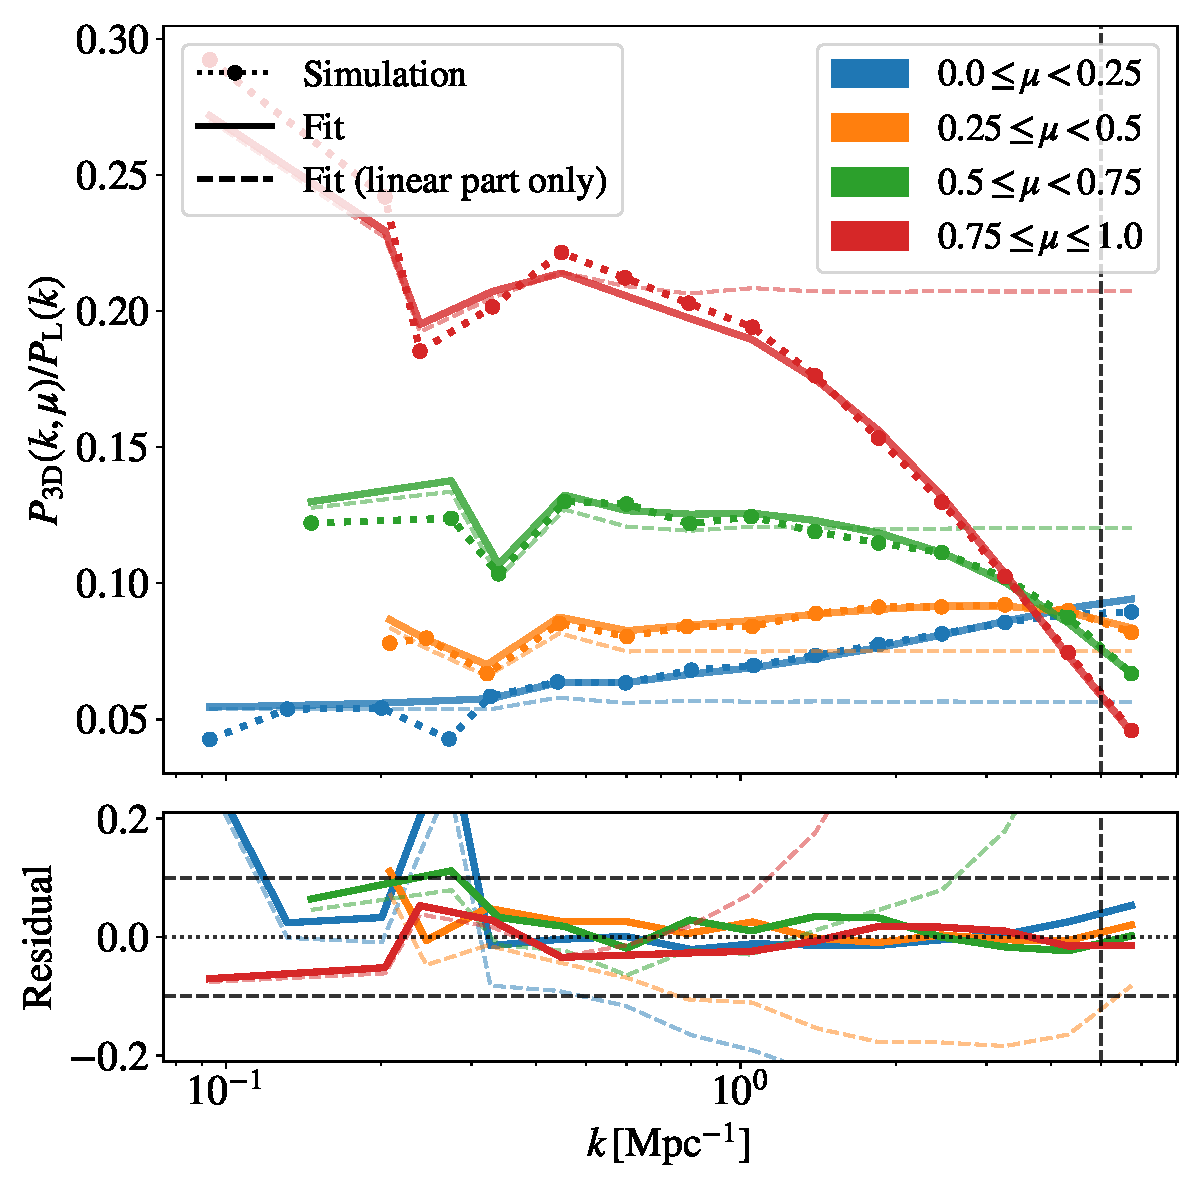
\includegraphics[width=\columnwidth]{figures/motivate.pdf}
\centering
\caption{Precision of the \pthreed model (see Eqs.~\ref{eq:p3d_model} and \ref{eq:dnl}) in reproducing measurements from the \simcentral simulation at $z=3$. \DIFdelbeginFL \DIFdelFL{The }\DIFdelendFL \DIFaddbeginFL \DIFaddFL{In the }\DIFaddendFL top panel\DIFdelbeginFL \DIFdelFL{shows }\DIFdelendFL \DIFaddbeginFL \DIFaddFL{, dotted and solid lines show }\DIFaddendFL the ratio of \DIFdelbeginFL %DIFDELCMD < \pthreed %%%
\DIFdelendFL \DIFaddbeginFL \DIFaddFL{simulation measurements and model predictions relative }\DIFaddendFL to the linear power spectrum\DIFdelbeginFL \DIFdelFL{: dotted lines represent simulation measurements}\DIFdelendFL , \DIFdelbeginFL \DIFdelFL{while solid and dashed }\DIFdelendFL \DIFaddbeginFL \DIFaddFL{respectively. Dashed }\DIFaddendFL lines \DIFdelbeginFL \DIFdelFL{indicate the ratio }\DIFdelendFL \DIFaddbeginFL \DIFaddFL{do so }\DIFaddendFL for the \DIFaddbeginFL \DIFaddFL{linear part of the }\DIFaddendFL best-fitting model \DIFdelbeginFL \DIFdelFL{with and without small-scale corrections, respectively}\DIFdelendFL \DIFaddbeginFL \DIFaddFL{($D_\mathrm{NL}=1$)}\DIFaddendFL . Line colors correspond to different $\mu$ wedges, and vertical dashed lines mark the minimum scale used for computing the best-fitting model, $k=5\iMpc$. The bottom panel displays the relative difference between the best-fitting model \DIFdelbeginFL \DIFdelFL{(with and without small-scale corrections) }\DIFdelendFL and simulation measurements. The overall precision of the model is 2\% on scales in which simulation measurements are not strongly affected by cosmic variance ($k>0.5\iMpc$; see text).
}
\label{fig:arinyo}
\end{figure}
%%%%%%%%%%%%%%%%%%%

We can express fluctuations in the \lyaf flux as $\delta_F(\mathbf{s}) = \bar{F}^{-1}(\mathbf{s}) F(\mathbf{s})-1$, where $F=\exp(-\tau)$ and $\bar{F}$ are the transmitted flux fraction and its mean, respectively, $\tau$ is the optical depth to \lya absorption, and $\mathbf{s}$ is the redshift-space coordinate. On linear scales, these fluctuations depend upon the matter field as follows \citep[e.g.;][]{mcdonald2003MeasurementCosmologicalGeometry} 
%
\begin{equation}
    \delta_F=b_\delta\, \delta + b_\eta\, \eta,
\end{equation}
%
where $\delta$ refers to matter density fluctuations, $\eta=-(a\,H)^{-1}(\partial v_\mathrm{r}/\partial r)$ stands for the dimensionless line-of-sight gradient of radial peculiar velocities, $a$ is the cosmological expansion factor, $H$ is the Hubble expansion factor, $v_\mathrm{r}$ is the radial velocity, and $r$ stands for the radial comoving coordinate. The linear bias coefficients $b_\delta$ and $b_\eta$ capture the response of $\delta_F$ to large-scale fluctuations in the $\delta$ and $\eta$ fields, respectively. 

Following \citet{mcdonald2003MeasurementCosmologicalGeometry}, we decompose the three-dimensional power spectrum of $\delta_F$ into three terms
%
\begin{equation}
    \label{eq:p3d_model}
    \pthreed(k,\,\mu) = (b_\delta + b_\eta\, f\, \mu^2)^2 D_\mathrm{NL}(k,\,\mu) P_\mathrm{lin}(k),
\end{equation}
%
where $f=\mathrm{d}\log G/\mathrm{d}\log a$ is the logarithmic derivative of the growth factor $G$, $(b_\delta + b_\eta\, f\, \mu^2)^2$ accounts for linear biasing and large-scale redshift space distortions \citep{kaiser1987ClusteringRealSpace, mcdonald2000ObservedProbabilityDistribution}, $P_\mathrm{lin}$ is the linear matter power spectrum\footnote{This is the linear power spectrum of cold dark matter and baryons even for cosmologies with massive neutrinos.}, and $D_\mathrm{NL}$ is a physically-motivated parametric correction accounting for the nonlinear growth of the density field, nonlinear peculiar velocities, thermal broadening, and pressure.

The large-scale behavior of \pthreed is set by the bias coefficients $b_\delta$ and $b_\eta$ together with the linear power spectrum, and the latter can be computed using a Boltzmann solver \citep[e.g.;][]{lewis2000EfficientComputationCosmic, lesgourgues2011CosmicLinearAnisotropy}. Therefore, the emulation of the 2 \lya linear biases enables predicting \pthreed on arbitrarily large (linear) scales\footnote{Aside from nonlinear effects affecting the position and damping of BAO.}. In contrast with direct emulation of power spectrum modes, this approach only requires simulations large enough for measuring the 2 \lya linear biases precisely.

Making predictions for \pthreed on small scales is more challenging than on large scales due to the variety of effects affecting this \DIFdelbegin \DIFdel{statistics }\DIFdelend \DIFaddbegin \DIFadd{statistic }\DIFaddend on the nonlinear regime \citep[e.g.;][]{mcdonald2003MeasurementCosmologicalGeometry}. In this work, we describe small-scale effects using the physically-motivated \citet{arinyo-i-prats2015NonlinearPowerSpectrum} parameterization
%
\begin{equation}
    \label{eq:dnl}
    D_\mathrm{NL} = \exp \left\{\left(q_1 \Delta^2 + q_2 \Delta^4\right) \left[1-\left(\frac{k}{k_\mathrm{v}}\right)^{a_\mathrm{v}} \mu^{b_\mathrm{v}}\right] - \left(\frac{k}{k_\mathrm{p}}\right)^2 \right\},
\end{equation}
%
where $\Delta^2(k)\equiv(2\uppi^2)^{-1} k^3 P_\mathrm{lin}(k)$ is the dimensionless linear matter power spectrum, $\mu$ is the cosine of the angle between the Fourier mode and the line of sight, and the free parameters $k_\mathrm{v}$ and $k_\mathrm{p}$ are in $\iMpc$ units throughout this work. The terms involving $\{q_1,\,q_2\}$, $\{k_\mathrm{v},\, a_\mathrm{v},\, b_\mathrm{v}\}$, and $\{k_\mathrm{p}\}$ account for nonlinear growth, peculiar velocities and thermal broadening, and gas pressure, respectively. \DIFdelbegin \DIFdel{Our emulator predicts the value of these 6 free parameters together with the 2 }%DIFDELCMD < \lya %%%
\DIFdel{linear biases}\DIFdelend \DIFaddbegin \DIFadd{In \mbox{%DIFAUXCMD
\citep{givans2022NonlinearitiesLymanAlpha}}\hspace{0pt}%DIFAUXCMD
, the authors used the previous expression to describe both }\pthreed \DIFadd{and }\poned \DIFadd{measurements down to highly nonlinear scales without the need for a shot-noise term. We will follow the same approach throughout this work; however, some authors advocate for such term \mbox{%DIFAUXCMD
\citep[e.g.;][]{irsicmcquinn2018}}\hspace{0pt}%DIFAUXCMD
}\DIFaddend .

In the top panel of Fig.~\ref{fig:arinyo}, \DIFdelbegin \DIFdel{we }\DIFdelend \DIFaddbegin \DIFadd{dotted lines }\DIFaddend show the ratio of \DIFdelbegin %DIFDELCMD < \pthreed %%%
\DIFdel{to }\DIFdelend \DIFaddbegin \DIFadd{measurements from the }\simcentral \DIFadd{simulation at $z=3$ and }\DIFaddend the linear power spectrum\DIFdelbegin \DIFdel{: dotted and solid lines indicate simulation measurements and }\DIFdelend \DIFaddbegin \DIFadd{, while solid lines do so for }\DIFaddend the best-fitting model to \DIFdelbegin \DIFdel{it }\DIFdelend \DIFaddbegin \DIFadd{these measurements }\DIFaddend (Eqs.~\ref{eq:p3d_model} and \ref{eq:dnl}) \DIFdelbegin \DIFdel{, respectively}\DIFdelend \DIFaddbegin \DIFadd{and the linear power spectrum}\DIFaddend . See \S\ref{sec:input} for details about this simulation and the fitting procedure. The dashed lines depict the results for the best-fitting model when setting $D_\mathrm{NL}=1$ after carrying out the fit; i.e., the \DIFdelbegin \DIFdel{behaviour }\DIFdelend \DIFaddbegin \DIFadd{behavior }\DIFaddend of the best-fitting model on linear scales. We can readily see that nonlinear growth isotropically increases the power with growing $k$, while peculiar velocities and thermal broadening suppress the power of parallel modes \DIFdelbegin \DIFdel{. On the smallest scalesshown}\DIFdelend \DIFaddbegin \DIFadd{as $k$ increases. On even smaller scales}\DIFaddend , pressure takes over and causes an isotropic suppression\DIFdelbegin \DIFdel{of all modes. These effects modify }\DIFdelend \DIFaddbegin \DIFadd{. Nonlinear growth modifies }\DIFaddend the perpendicular power \DIFaddbegin \DIFadd{relative to linear theory }\DIFaddend by 10\% for scales as large as $k=0.5\iMpc$, indicating that small-scale corrections \DIFdelbegin \DIFdel{affect }\DIFdelend \DIFaddbegin \DIFadd{are important for }\DIFaddend most of the scales sampled by our simulations. Nevertheless, our simulations are large enough to measure the 2 \lya linear biases with percent precision (see Appendix~\ref{sec:cosmic_variance}). \DIFaddbegin \DIFadd{Deviations from linear theory are less pronounced down to smaller scales for modes with $\mu\simeq0.5$ because nonlinear growth and the combination of peculiar velocities and thermal broadening tend to cancel each other out.
}\DIFaddend 

On the largest scales, we find strong variations between consecutive $k$-bins for the same $\mu$-wedge. Some of these oscillations are driven by differences in the average value of $\mu$ between consecutive bins due to the limited number of modes entering each bin on large scales. To ensure an accurate comparison between simulation measurements and model predictions, we individually evaluate the \pthreed model for all the modes within each $k-\mu$ bin from our simulation boxes. We then calculate the mean of the resulting distribution and assign this mean value to the bin, thereby mirroring the approach used to compute \pthreed measurements from the simulations. This process is crucial for large scales where the number of modes is small and nonlinear scales where the dependence of the number of modes with $k$ is strong. We follow the same approach to evaluate the \pthreed model throughout this work.

After accounting for the previous effect, the best-fitting model reproduces most large-scale oscillations. However, we can readily see a fluctuation at $k\simeq0.25\iMpc$ in the $0<\mu<0.25$ wedge that it is not captured by the model. The difference between model predictions and simulation measurements for the bins adjacent to this one is approximately zero, suggesting that this fluctuation is caused by cosmic variance. We characterize the impact of this source of uncertainty in Appendix~\ref{sec:cosmic_variance}, concluding that it can induce up to 10\% errors on scales larger than $k=0.5\iMpc$. Consequently, cosmic variance hinders our ability to evaluate the model's performance on the largest scales shown. However, this does not necessarily indicate a decrease in model precision on scales larger than $k=0.5\iMpc$; rather, our simulations are simply not large enough to accurately assess the model's precision on such scales. In the bottom panel of Fig.~\ref{fig:arinyo}, we can see that the average precision of the model is 2\% for $k>0.5\iMpc$, supporting the use of Eq.~\ref{eq:dnl} for capturing small-scale deviations from linear theory.

%%%%%%%%%%%%%%%%%%%%
%%%%%%%%%%%%%%%%%%%%

\subsection{Input and output parameters}
\label{sec:strategy_params}

In addition to the density and velocity fields, the \lyaf depends upon the ionization and thermal state of the IGM \citep[e.g.;][]{mcdonald2003MeasurementCosmologicalGeometry}. Following \citet{Pedersen2021}, we use 6 parameters to describe the dependency of this observable with cosmology and IGM physics:

\begin{itemize}
    \item Amplitude ($\Delta^2_\mathrm{p}$) and slope ($n_\mathrm{p}$) of the linear matter power spectrum on small scales. These are defined as
    %
    \begin{align}
        \label{eq:amplitude}
        & \Delta_\mathrm{p}^2(z) = \DIFaddbegin \DIFadd{(2\pi^2)^{-1} }\DIFaddend k^3 P_{\rm lin} (k_\mathrm{p}, z),\\
        \label{eq:slope}
        & n_\mathrm{p}(z) = \left(\mathrm{d}\log P_{\rm lin} / \mathrm{d}\log k\right)\mid_{k = k_\mathrm{p}},
    \end{align}
    %
    where we use $k_\mathrm{p} = 0.7\,\mathrm{Mpc}^{-1}$ as the pivot scale because it is at the center of the range of interest for DESI small-scale studies. These parameters capture multiple physical effects modifying the linear power spectrum on small scales \citep[see][for a detailed discussion]{Pedersen2021}, including cosmological parameters such as the amplitude ($A_\mathrm{s}$) and slope ($n_\mathrm{s}$) of the primordial power spectrum, the Hubble parameter, and the matter density (\DIFdelbegin \DIFdel{$\Omega_\mathrm{m}$}\DIFdelend \DIFaddbegin \DIFadd{$\Omega_\mathrm{M}$}\DIFaddend ), or $\Lambda$CDM extensions such as curvature and massive neutrinos. The advantage of using this parameterization rather than $\Lambda$CDM parameters is twofold. First, we reduce the dimensionality of the emulator input, which decreases the number of simulations required for precise training. Second, the resulting emulator has the potential for making precise predictions for variations in cosmological parameters and $\Lambda$CDM extensions not considered in the training set \citep[][]{Pedersen2021, pedersen2023CompressingCosmologicalInformation, cabayol-garcia2023NeuralNetworkEmulator}. Note that we do not consider cosmological parameters capturing changes in the growth rate or expansion history because the \lyaf probes cosmic times during which the universe is practically Einstein de-Sitter, and both vary very little with cosmology in this regime.

    \item Mean transmitted flux fraction (\mflux). It depends on the intensity of the cosmic ionizing background and evolves strongly with redshift. One of the advantages of using this parameter is that it encodes the majority of the redshift dependence of the signal, serving as a proxy for cosmic time.

    \item Amplitude and slope of the temperature-density relation. The thermal state of the IGM can be approximated by a power law on the densities probed by the \lyaf \citep{hydro_Lukic2015}: \DIFdelbegin \DIFdel{$T_0\Delta_\mathrm{b}^\gamma$}\DIFdelend \DIFaddbegin \DIFadd{$T_0\Delta_\mathrm{b}^{\gamma-1}$}\DIFaddend , where $\Delta_\mathrm{b}$ is the baryon overdensity, $T_0$ is the gas temperature at mean density, and \DIFdelbegin \DIFdel{$\gamma$ }\DIFdelend \DIFaddbegin \DIFadd{$\gamma-1$ }\DIFaddend is the slope of the relation. These parameters influence the ionization of the IGM, which is captured by \mflux, and the thermal motion of gas particles, which causes Doppler broadening that suppresses the parallel power. Instead of using $T_0$ as an emulator parameter, we follow \citet{Pedersen2021} and use the thermal broadening scale in comoving units. First, we express the thermal broadening in velocity units as $\tilde{\sigma}_\mathrm{T} = 9.1 (T_0[\mathrm{K}]/10^4)^{1/2}$, and then we convert it to comoving units, $\sigma_\mathrm{T}=\tilde{\sigma}_\mathrm{T}(1+z) H^{-1}$.

    \item Pressure smoothing scale. Gas pressure supports baryons on small scales, leading to a strong isotropic power suppression in this regime. The characteristic smoothing scale depends upon the entire thermal history of the gas \citep{gnedin1998ProbingUniverseLyalpha}, and we parameterize its effect using the pressure smoothing scale in comoving units of Mpc$^{-1}$, $k_\mathrm{F}$ (see \citet{Pedersen2021} for more details).
\end{itemize}

Our emulator predicts the 8 free parameters of the \pthreed model introduced by Eqs.~\ref{eq:p3d_model} and \ref{eq:dnl}, $\mathbf{y}=\{b_\delta,\, b_\eta,\, q_1,\, q_2,\, k_\mathrm{v},\, a_\mathrm{v},\, b_\mathrm{v}, \, k_\mathrm{p}\}$, as a function of the previous 6 parameters, $\mathbf{x}=\{\Delta_\mathrm{p}^2,\, n_\mathrm{p},\, \mflux,\, \sigma_\mathrm{T},\, \gamma,\, k_\mathrm{F}\}$. In the three next sections, we generate the training data of the emulator, discuss its implementation, and evaluate its precision.

%%%%%%%%%%%%%%%%%%%%
%%%%%%%%%%%%%%%%%%%%
%%%%%%%%%%%%%%%%%%%%

\section{Training and testing set}
\label{sec:input}

In this section, we describe how we generate the training and testing data of our emulator. In \S\ref{sec:input_sims}, we present a suite of cosmological hydrodynamical simulations from which we generate mock \lyaf measurements, and we detail our approach for extracting \pthreed and \poned measurements from these simulations in \S\ref{sec:input_extract_lya}. In \S\ref{sec:input_fitting}, we compute the best-fitting parameters of the model introduced by Eqs.~\ref{eq:p3d_model} and \ref{eq:dnl} to measurements of these statistics, and we evaluate the performance of the fits in \S\ref{sec:input_precision}.

%%%%%%%%%%%%%%%%%%%%
%%%%%%%%%%%%%%%%%%%%

\subsection{Simulations}
\label{sec:input_sims}

We extract \lyaf measurements from a suite of simulations run with \textsc{mp-gadget}\footnote{\url{https://github.com/MP-Gadget/MP-Gadget/}} \citep{feng2018MpGadgetMpGadgetTag, emugp_bird2019}, a massively scalable version of the cosmological structure formation code \textsc{gadget-3} \citep[last described in][]{Gadget_Springel}. This suite of simulations was first presented and used in \citet{Pedersen2021}; we briefly describe it next. Each simulation tracks the evolution of $768^3$ dark matter and baryon particles from $z=99$ to $z=2$ inside a box of $L = 67.5$ Mpc on a side, producing as output 11 snapshots uniformly spaced in redshift between $z=4.5$ and 2. \DIFaddbegin \DIFadd{This configuration ensures convergence for }\poned \DIFadd{measurements down to $k_\parallel=4\iMpc$ (the smallest scale used in this work) at $z=2$ and less than 10\% errors for this scale at $z=4$. For more details, see the box size and mass resolution tests carried out in \mbox{%DIFAUXCMD
\citet{bolton2017SherwoodSimulationSuite}}\hspace{0pt}%DIFAUXCMD
.
}

\DIFaddend Two realizations were run for each combination of cosmological and astrophysical parameters using the ``fixed-and-paired'' technique \citep{angulo2016CosmologicalNbodySimulations, pontzen2016InvertedInitialConditions}, which significantly reduces cosmic variance for multiple observables, including the \lyaf \citep{fixedpaired_Villaescusa, anderson2019CosmologicalHydrodynamicSimulations}. \DIFaddbegin \DIFadd{The initial conditions were generated using the following configuration of }\textsc{\DIFadd{mp-genic}} \DIFadd{\mbox{%DIFAUXCMD
\citep{Bird2020}}\hspace{0pt}%DIFAUXCMD
: initial displacements produced using the Zel'dovich approximation and baryons and dark matter initialized on an offset grid using species-specific transfer functions. Some studies have suggested that this configuration might lead to incorrect evolution of linear modes \mbox{%DIFAUXCMD
\citep{Bird2020}}\hspace{0pt}%DIFAUXCMD
. However, in a recent study, \mbox{%DIFAUXCMD
\citet{Khan2024} }\hspace{0pt}%DIFAUXCMD
showed that variations in the specific settings of }\textsc{\DIFadd{mp-genic}} \DIFadd{initial conditions have a minimal impact on }\poned \DIFadd{measurements across the range of redshifts and scales used in this work.
}\DIFaddend 

To increase computational efficiency, the simulations utilize a simplified prescription for star formation that turns regions of baryon overdensity $\Delta_\mathrm{b}>1000$ and temperature $T<10^5$ K into collisionless stars \citep[e.g.;][]{viel2004ConstraintsPrimordialPower}, implement a spatially uniform ultraviolet background \citep{haardt2012RadiativeTransferClumpya}, and do not consider active galactic nuclei (AGN) feedback \citep[e.g.;][]{chabanier2020ImpactAGNFeedback}. These approximations are justified because we focus on emulating the \lyaf in the absence of astrophysical contaminants like AGN feedback, damped Lyman-alpha absorbers (DLAs), or metal absorbers, and we will model these before comparing our predictions with observational measurements \citep[e.g.;][]{mcdonald2005LinearTheoryPower, palanque-delabrouille2015ConstraintNeutrinoMasses, palanque-delabrouille2020HintsNeutrinoBounds}.

We train \forestflow using data from 30 fixed-and-paired simulations spanning combinations of cosmological and astrophysical parameters selected according to a Latin hypercube \citep{mckay1979ComparisonThreeMethods}; we refer to these as \lacehc simulations hereafter. The Latin hypercube spans the parameters \DIFdelbegin \DIFdel{$\{\Delta^2_\mathrm{p}(z=z_\star),\, n_\mathrm{p}(z=z_\star),\, z_\mathrm{H},\, H_\mathrm{A},\, H_\mathrm{S}\}$}\DIFdelend \DIFaddbegin \DIFadd{$\{\Delta^2_\mathrm{p}(z=3),\, n_\mathrm{p}(z=3),\, z_\mathrm{H},\, H_\mathrm{A},\, H_\mathrm{S}\}$}\DIFaddend , where we use \DIFdelbegin \DIFdel{$z_\star=3$ }\DIFdelend \DIFaddbegin \DIFadd{$z=3$ }\DIFaddend because it is approximately at the center of the range of interest for DESI studies \citep{ravoux2023DarkEnergySpectroscopica, karacayli2024Optimal1DLy}, $z_\mathrm{H}$ is the midpoint of hydrogen reionization, and the last two parameters rescale the \ion{He}{ii} photoheating rate $\epsilon_0$ as $\epsilon = H_\mathrm{A} \Delta_\mathrm{b}^{H_\mathrm{S}} \epsilon_0$ \citep{onorbe2017SelfconsistentModelingReionization}. Cosmological parameters were generated within the ranges \DIFdelbegin \DIFdel{$\Delta^2_\mathrm{p}(z=z_\star) \in [0.25,\, 0.45]$, $n_\mathrm{p}(z=z_\star) \in [-2.35,\, -2.25]$ }\DIFdelend \DIFaddbegin \DIFadd{$\Delta^2_\mathrm{p}(z=3) \in [0.25,\, 0.45]$, $n_\mathrm{p}(z=3) \in [-2.35,\, -2.25]$ }\DIFaddend by exploring values of the amplitude and slope of the primordial power spectrum within the intervals $A_\mathrm{s} \in [1.35,\, 2.71]\times 10^{-9}$ and $n_\mathrm{s} \in [0.92,\, 1.02]$. Any other $\Lambda$CDM parameter was held fixed to approximately \citet{planckcollaboration2020Planck2018Resultsa} values: dimensionless Hubble parameter $h=0.67$, physical cold dark matter density $\Omega_\mathrm{c} h^2=0.12$, and physical baryon density $\Omega_\mathrm{b} h^2=0.022$. As for the IGM parameters, these explored the ranges $z_\mathrm{H}\in[5.5,\,15]$, $H_\mathrm{A}\in[0.5,\,1.5]$, and $H_\mathrm{S}\in[0.5,\,1.5]$. All simulation pairs use the same set of initial Fourier phases, and thus cosmic variance affects in approximately the same way all combinations of input parameters.

We evaluate different aspects of the emulation strategy using 6 fixed-and-paired simulations with cosmological and astrophysical parameters not considered in the \lacehc simulations:
%
\begin{itemize}
    \item The \simcentral simulation uses cosmological and astrophysical parameters at the center of the \lacehc parameter space\DIFaddbegin \DIFadd{: $A_\mathrm{s}=2.01\times10^{-9}$, $n_\mathrm{s}=0.97$, $z_\mathrm{H}=10.5$, $H_\mathrm{A}=1$, and $H_\mathrm{S}=1$}\DIFaddend . We use this simulation for an out-of-sample test of the emulator's performance under optimal conditions, as the precision of machine-learning models typically decreases as we move closer to the border of the convex hull set by the training set.

    \item The \simseed simulation uses the same parameters as the \simcentral simulation while considering a different distribution of initial Fourier phases. Given that all \lacehc simulations use the same initial Fourier phases, \simseed is useful to evaluate the impact of cosmic variance in the training set on \forestflow predictions.

    \item The \simh, \simnu, and \simcurved simulations adopt the same values of \DIFdelbegin \DIFdel{$\Delta^2_\mathrm{p}(z_\star)$, $n_\mathrm{p}(z_\star)$}\DIFdelend \DIFaddbegin \DIFadd{$\Delta^2_\mathrm{p}(z=3)$, $n_\mathrm{p}(z=3)$}\DIFaddend , physical cold dark matter and baryonic densities, and astrophysical parameters as the \simcentral simulation. However, the \simh simulation uses 10\% larger Hubble parameter ($h=0.74$) and 18\% smaller matter density (\DIFdelbegin \DIFdel{$\Omega_\mathrm{m}=0.259$}\DIFdelend \DIFaddbegin \DIFadd{$\Omega_\mathrm{M}=0.259$}\DIFaddend ) while using the same value of \DIFdelbegin \DIFdel{$\Omega_\mathrm{m} h^2$ }\DIFdelend \DIFaddbegin \DIFadd{$\Omega_\mathrm{M} h^2$ }\DIFaddend as the \lacehc simulations, the \simnu simulation includes massive neutrinos ($\sum m_\nu=0.3$ eV), and the \simcurved simulation considers an open universe ($\Omega_k=0.03$). The \simnu and \simcurved simulations also modify the value of the cosmological constant while holding fixed $h$ to compensate for the increase in the matter density and the addition of curvature, respectively. The testing simulations address the precision of the emulation strategy for cosmologies not included in the training set.

    \item The \simigm simulation uses the same cosmological parameters as the \simcentral simulation while implementing a distinct helium ionization history relative to the \simcentral and \lacehc simulations \citep{puchwein2019ConsistentModellingMetagalactic}. The main difference between the ionization histories of these simulations is that the one implemented in the \simigm simulation peaks at a later time than the others, leading to a significantly different thermal history. The \simigm simulation therefore tests the emulator's performance for thermal histories not considered in the \lacehc simulations.
\end{itemize}

%%%%%%%%%%%%%%%%%%%%
%%%%%%%%%%%%%%%%%%%%

\subsection{Simulating \lyaf data}
\label{sec:input_extract_lya}

To extract \lyaf measurements from each simulation, we first select one of the simulation axes as the line of sight and displace the simulation particles from real to redshift space along this axis. Then, we compute the transmitted flux fraction along $768^2$ uniformly-distributed line of sights along this axis using \textsc{FSFE}\footnote{\url{https://github.com/sbird/fake_spectra}.} \citep{bird2017FSFEFakeSpectra}; these lines of sight are commonly known as skewers. The resolution of the skewers is set to 0.05 Mpc, which is enough to resolve the thermal broadening and pressure scales, and are spaced by 0.09 Mpc in the transverse direction. We checked that \pthreed and \poned measurements within the range of interest (see \S\ref{sec:input_fitting}) do not vary by increasing the line-of-sight resolution or the transverse sampling. After that, we repeat the previous steps for the three simulation axes to extract further cosmological information, as each simulation axis samples the velocity field in a different direction. Finally, we scale the effective optical depth of the skewers to 0.90, 0.95, 1.05, and 1.10 times its original value \citep[see][for more details about this approach]{hydro_Lukic2015}, which is equivalent to running simulations with different values of the UV background.

Using this data as input, we measure \pthreed by first computing the three-dimensional Fourier transform of the skewers. Then, we take the average of the square norm of all modes within 20 logarithmically-spaced bins in wavenumber $k$ from the fundamental mode of the box, $k_\mathrm{min}=2\uppi L^{-1} \simeq 0.09\iMpc$, to $k_\mathrm{max}=40\iMpc$ and 16 linearly-spaced bins in the cosine of the angle between Fourier modes and the line of sight from $\mu=0$ to 1. We measure \poned by first computing the one-dimensional Fourier transform of each skewer without applying any binning, and then by taking the average of the square norm of all these Fourier transforms.

We carry out these measurements for the 30 \lacehc and 6 test fix-and-paired simulations, ending up with 2 (opposite Fourier phases) $\times$ 3 (simulation axes) $\times$ 11 (snapshots) $\times$ 5 (mean flux rescalings) $=330$ measurements per simulation. To reduce cosmic variance, we compute the average of measurements from different axes and phases of fixed-and-paired simulations, decreasing the number of measurements per simulation to 55. The training and testing sets of \forestflow are thus comprised of 1650 and 330 \lya power spectrum measurements, respectively. All these measurements are publicly available at \url{https://github.com/igmhub/LaCE}.

%%%%%%%%%%%%%%%%%%%
%%%%%%%%%%%%%%%%%%%

\subsection{Fitting the parametric model}
\label{sec:input_fitting}

To generate training and testing data for our emulator, we compute the best-fitting parameters of Eqs.~\ref{eq:p3d_model} and ~\ref{eq:dnl} to measurements from the simulations described in \S\ref{sec:input_sims}. We fit the model using \pthreed measurements from $k=0.09$ to $5\iMpc$ and \poned measurements from $k_\parallel=0.09$ to $4\iMpc$. The size of our simulation boxes determines the largest scales used, while the maximum wavenumbers are set by the smallest scales measured by \citep{ravoux2023DarkEnergySpectroscopica, karacayli2024Optimal1DLy}. We remind the reader that the large-scale behavior of \pthreed is set by the 2 \lya linear biases (see Eq.~\ref{eq:p3d_model}); consequently, the model can make accurate predictions for \pthreed on arbitrarily large (linear) scales as long as these 2 parameters are measured precisely.

We compute the best-fitting value of model parameters $\mathbf{y}=\{b_\delta,\, b_\eta,\, q_1,\, q_2,\, k_\mathrm{v},\, a_\mathrm{v},\, b_\mathrm{v}, \, k_\mathrm{p}\}$ to simulation measurements by minimizing the pseudo-$\chi^2$:
%
\begin{align}
    \label{eq:chi2}
    \chi^2(\mathbf{y}) =& \,\,\sum_{i}^{M_\mathrm{3D}} w_\mathrm{3D}\left[P_\mathrm{3D}^\mathrm{data}(k_i, \mu_i) - P_\mathrm{3D}^\mathrm{model}(k_i, \mu_i, \mathbf{y})\right]^2 \nonumber\\ 
    +&\,\, \sum_{i}^{M_\mathrm{1D}} w_\mathrm{1D} 
    \left[P_\mathrm{1D}^\mathrm{data}(k_{\parallel,\,i}) - P_\mathrm{1D}^\mathrm{model}(k_{\parallel,\,i}, \mathbf{y})\right]^2,
\end{align}
%
where $M_\mathrm{3D}=164$ and $M_\mathrm{1D}=42$ are the number of \pthreed and \poned bins employed in the fit, respectively, the superscripts data and model refer to simulation measurements and model predictions, and $w_\mathrm{3D}$ and $w_\mathrm{1D}$ weigh the fit. We use the Nelder-Mead algorithm implemented in the routine {\sc minimize} of {\sc scipy} \citep{virtanen2020_SciPyFundamentalalgorithms} to carry out the minimization \footnote{To ensure that this routine does not get stuck in a local minimum, we checked that the likelihood is unimodal in all cases using the Affine Invariant Markov chain Monte Carlo Ensemble sampler \textsc{emcee} \citep{foremanmackey13}.}. The results of the fits are publicly accessible at \url{https://github.com/igmhub/ForestFlow}.

Ideally, we would use the covariance of \pthreed and \poned measurements as weight in the previous expression; however, we lack multiple realizations of the same simulation with different distributions of initial Fourier phases needed to estimate this covariance. In addition, its theoretical estimation is not straightforward \citep{maion2022fpvariance}. Instead, we disregard correlations between \pthreed and \poned and weigh these by $w_\mathrm{3D}= N_\mathrm{3D}(k, \mu)/(1+\mu^2)^2$ and $w_\mathrm{1D}=\alpha (1+k_{\parallel}/k_0)^2$, where $N_\mathrm{3D}$ is the number of modes in each $k-\mu$ bin and $k_0=2\iMpc$. The terms involving $N_\mathrm{3D}$, $\mu$, and $k_0$ attempt to ensure an unbiased fit of \pthreed and \poned across the full range of scales used. The parameter $\alpha=8000$ controls the relative weight of \pthreed and \poned in the fit, and its value is motivated by the different impact of cosmic variance on these (see Appendix~\ref{sec:cosmic_variance}).

We expect significant correlations between the best-fitting value of the parameters to measurements from relatively small simulation boxes. As shown by \citet{arinyo-i-prats2015NonlinearPowerSpectrum}, these correlations are especially significant for the parameters accounting for nonlinear growth of structure, $q_1$ and $q_2$. \citet{givans2022NonlinearitiesLymanAlpha} advocated for setting $q_2=0$ since this parameter is not necessary for describing \pthreed at $z=2.8$. However, we find non-zero values of this parameter indispensable for describing \pthreed at redshifts below $z=2.5$. This is not surprising since the gravitational evolution of density perturbations becomes increasingly more nonlinear as cosmic time progresses.


%%%%%%%%%%%%%%%%%%%
%%%%%%%%%%%%%%%%%%%


%%%%%%%%%%%%%%%%%%%
\begin{figure}
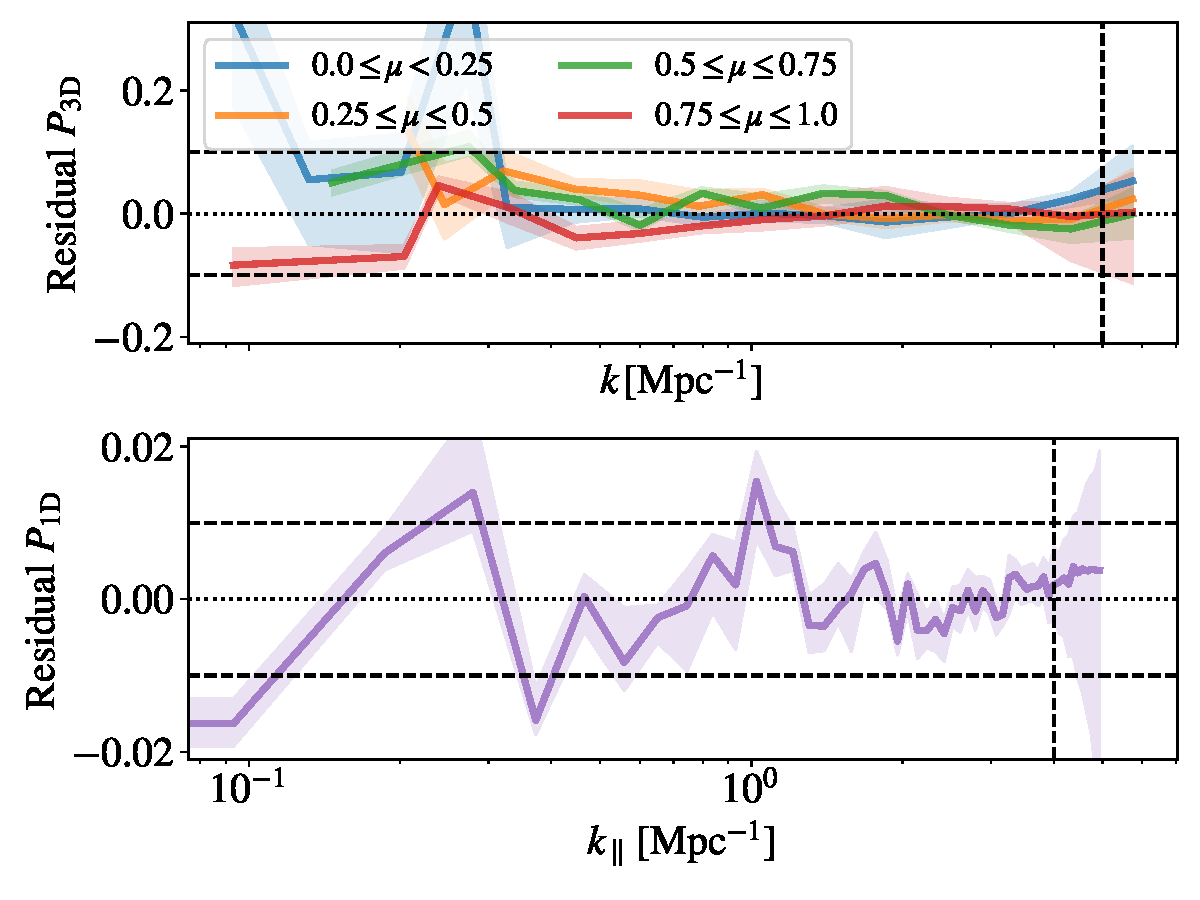
\includegraphics[width=\columnwidth]{figures/goodness_fit_all.pdf}
\centering
\caption{Precision of the parametric model (see Eqs.~\ref{eq:p3d_model} and \ref{eq:dnl}) in reproducing \pthreed and \poned measurements from all the \lacehc simulations. Lines and shaded areas show the mean and standard deviation of the relative difference between simulation measurements from the 1650 snapshots of the \lacehc simulations and best-fitting models to these, respectively. The precision of the model in recovering \pthreed and \poned is 2.4 and 0.6\%, respectively, on scales not strongly affected by cosmic variance.}
\label{fig:goodness}
\end{figure}
%%%%%%%%%%%%%%%%%%%

\subsection{Precision of the model}
\label{sec:input_precision}

In the previous section, we compute the best-fitting parameters of the \pthreed model to measurements from the \lacehc simulations. Two main sources of uncertainty can affect these fits: \DIFdelbegin \DIFdel{cosmic variance and model inaccuracies }\DIFdelend \DIFaddbegin \DIFadd{model inaccuracies and cosmic variance}\DIFaddend . The first \DIFaddbegin \DIFadd{relates to using a model with a limited number of free parameters to describe }\lya \DIFadd{clustering, while the second }\DIFaddend comes from the limited size of the \lacehc simulations\DIFdelbegin \DIFdel{, and it }\DIFdelend \DIFaddbegin \DIFadd{. In our case, cosmic variance }\DIFaddend is amplified because \DIFdelbegin \DIFdel{they all }\DIFdelend \DIFaddbegin \DIFadd{all the }\lacehc \DIFadd{simulations }\DIFaddend use the same initial distribution of Fourier phases, meaning all simulations are subject to the same large-scale noise. We study this source of uncertainty in Appendix~\ref{sec:cosmic_variance}, where we compare the best-fitting models to two simulations whose only difference is in their initial distribution of Fourier phases. \DIFdelbegin \DIFdel{Cosmic variance causes differences of 0.6 and 1.8\% on the value of $b_\delta$ and $b_\eta$ --- equivalent to 1.2 and 1.8\% for perpendicular and parallel }%DIFDELCMD < \pthreed %%%
\DIFdel{modes on linear scales --- and 0.8 and 0.1\% on predictions for }%DIFDELCMD < \pthreed %%%
\DIFdel{and }%DIFDELCMD < \poned %%%
\DIFdel{from the best-fitting models, respectively, throughout the range of scales used in the fits. The second relates to using a parametric model with a limited number of free parameters to describe }%DIFDELCMD < \lya %%%
\DIFdel{clustering}\DIFdelend \DIFaddbegin \DIFadd{We proceed to study model inaccuracies next}\DIFaddend .

In Fig.~\ref{fig:goodness}, we evaluate the performance of the parametric model in reproducing \pthreed and \poned measurements from the 1650 snapshots of the \lacehc simulations. As discussed in \S\ref{sec:strategy_model}, cosmic variance \DIFdelbegin \DIFdel{hinders }\DIFdelend \DIFaddbegin \DIFadd{limits }\DIFaddend our ability to evaluate the precision of the model for \pthreed on scales larger than $k=0.5\iMpc$; \DIFdelbegin \DIFdel{motivated by this, we do so }\DIFdelend \DIFaddbegin \DIFadd{therefore, we quote the model precision }\DIFaddend from this scale \DIFaddbegin \DIFadd{down }\DIFaddend to the smallest \DIFdelbegin \DIFdel{one }\DIFdelend \DIFaddbegin \DIFadd{scale }\DIFaddend used in the fit, $k=5\iMpc$. \DIFdelbegin \DIFdel{On the other hand, since the impact of cosmic variance on }%DIFDELCMD < \poned %%%
\DIFdel{is much smaller , we estimate }\DIFdelend \DIFaddbegin \DIFadd{In contrast, since cosmic variance has a much smaller impact on }\poned\DIFadd{, we evaluate }\DIFaddend the model performance for this statistic using all scales considered in the fit, $0.09<k_\parallel[\iMpc]<4$. We \DIFdelbegin \DIFdel{will follow }\DIFdelend \DIFaddbegin \DIFadd{adopt }\DIFaddend the same approach when evaluating the precision of the emulator in \S\ref{sec:results}. Under these considerations, the overall precision of the model \DIFdelbegin \DIFdel{in recovering }%DIFDELCMD < \pthreed %%%
\DIFdel{and }%DIFDELCMD < \poned %%%
\DIFdelend is 2.4 and 0.6\% \DIFaddbegin \DIFadd{for }\pthreed \DIFadd{and }\poned\DIFaddend , respectively. 
\DIFaddbegin 

\DIFaddend Given that we estimate the precision of the model using our simulations, \DIFdelbegin \DIFdel{these }\DIFdelend \DIFaddbegin \DIFadd{the previous }\DIFaddend numbers account for both the limited flexibility of the \pthreed model and cosmic variance. \DIFdelbegin \DIFdel{The impact of the second on }\DIFdelend \DIFaddbegin \DIFadd{As discussed in Appendix~\ref{sec:cosmic_variance}, the impact of cosmic variance on measurements of }\DIFaddend \pthreed and \poned \DIFdelbegin \DIFdel{measurements }\DIFdelend from our simulations is 1.3 and 0.5\%, respectively\DIFdelbegin \DIFdel{, across the previous range of scales (see Appendix~\ref{sec:cosmic_variance}). The precision for }%DIFDELCMD < \poned %%%
\DIFdel{is practically the same in both cases and less than 1\% worse for }\DIFdelend \DIFaddbegin \DIFadd{. This indicates that the limited flexibility of the }\DIFaddend \pthreed \DIFdelbegin \DIFdel{, letting us }\DIFdelend \DIFaddbegin \DIFadd{model introduces additional errors of 1.1 and 0.1\% on these statistics beyond cosmic variance. We can thus }\DIFaddend conclude that the \pthreed model \DIFdelbegin \DIFdel{reproduces both statistics accurately }\DIFdelend \DIFaddbegin \DIFadd{accurately reproduces }\pthreed \DIFadd{and }\poned \DIFadd{over the full range of scales used in the fit, $0.09<k[\iMpc]<5$ and $0.09<k_\parallel[\iMpc]<4$}\DIFaddend .

%%%%%%%%%%%%%%%%%%%%
%%%%%%%%%%%%%%%%%%%%
%%%%%%%%%%%%%%%%%%%%

%%%%%%%%%%%%%%%%%%%%
\begin{figure*}
    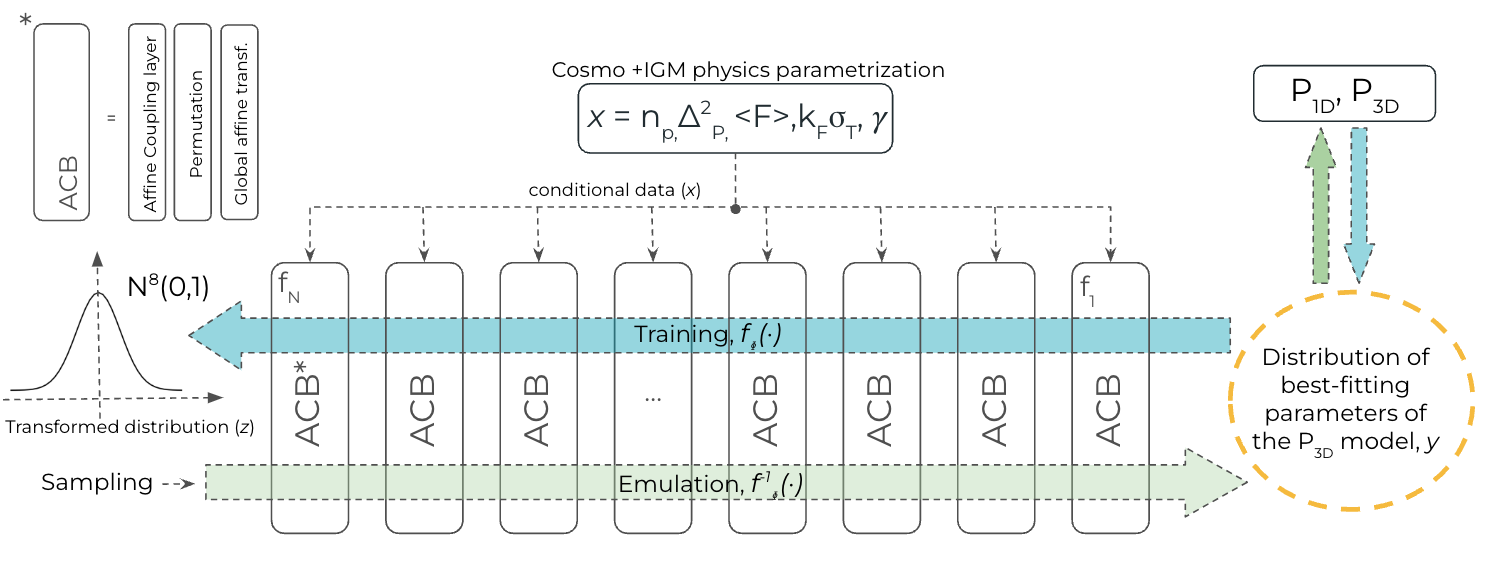
\includegraphics[width= 0.98\textwidth]{figures/network_architecture.png} 
    \centering
    \caption{Architecture of \forestflow, a \lyaf emulator based on conditional Normalizing Flows. The blue arrow indicates the training direction, where \forestflow optimizes a bijective mapping between the best-fitting parameters of the \pthreed model to measurements from the \lacehc simulations and an 8-dimensional Normal distribution. The mapping is conditioned on cosmology and IGM physics and performed using 12 consecutive affine coupling blocks. The green arrow denotes the emulation direction, where the emulator applies the inverse of the mapping to random samples from the base distribution to predict the value of the \pthreed model parameters. Outside the cNF, \forestflow introduces these parameters in Eq.~\ref{eq:p3d_model} and \ref{eq:p1d} to obtain predictions for \pthreed and \poned, respectively.}
    \label{fig:net_architecture}
 \end{figure*}
%%%%%%%%%%%%%%%%%%%%

\section{ForestFlow}
\label{sec:forestflow}

In this section we present \forestflow, an emulator based on conditional normalizing flows that predicts the parameters of the \pthreed model introduced by Eqs.~\ref{eq:p3d_model} and \ref{eq:dnl} as a function of parameters capturing the dependence of the \lyaf on cosmology and IGM physics. We detail its architecture and implementation in \S\ref{sec:forestflow_NF} and \ref{sec:forestflow_implementation}, respectively.

%%%%%%%%%%%%%%%%%%%%
%%%%%%%%%%%%%%%%%%%%

\subsection{Conditional normalizing flows}
\label{sec:forestflow_NF}

Normalizing flows \citep[NFs;][]{NF_Rezende2015} are a class of machine-learning generative models designed to predict complex distributions by applying a sequence of bijective mappings to simple base distributions. A natural extension to this framework is conditional NFs \citep[cNFs;][]{Winkler2019, cNF_Papamakarios}, a type of NFs that condition the mapping between the base and target distributions on a series of input variables. Given an input $\mathbf{x} \in X$ and target $\mathbf{y} \in Y$, cNFs predict the conditional distribution $p_{Y|X}(\mathbf{y}|\mathbf{x})$ by applying a parametric, bijective mapping $f_\phi: Y\times X \to Z$ to a base distribution $p_{Z}(\mathbf{z})$ as follows
%
\begin{equation}
    \label{eq:cNF_pdf}
    p_{Y|X}(\mathbf{y}|\mathbf{x}) = p_{Z}(f_\phi(\mathbf{y}, \mathbf{x})|\mathbf{x}) \left|\frac{\partial f_\phi(\mathbf{y}, \mathbf{x})}{\partial \mathbf{y}}\right|,
\end{equation}
%
where $\phi$ are the parameters of the mapping, while the last term of the previous equation is the Jacobian determinant of the mapping. In \forestflow, the input is given by the parameters capturing the dependence of the \lyaf on cosmology and IGM physics, $\mathbf{x}=\{\Delta_\mathrm{p}^2,\, n_\mathrm{p},\, \mflux,\, \sigma_\mathrm{T},\, \gamma,\, k_\mathrm{F}\}$, the target by the parameters of the \pthreed model, $\mathbf{y}=\{b_\delta,\, b_\eta,\, q_1,\, q_2,\, k_\mathrm{v},\, a_\mathrm{v},\, b_\mathrm{v}, \, k_\mathrm{p}\}$, and the base distribution is an 8-dimensional Normal distribution $N^8(0,1)$, where the dimension is determined by the number of \pthreed model parameters.

Once trained, cNFs are a generative process from $\mathbf{x}$ to $\mathbf{y}$. In our implementation, \forestflow first samples randomly from the base distribution, and then it passes this realization through a sequence of mappings conditioned on a particular combination of cosmology and IGM parameters, $\mathbf{\tilde{y}}=f_\phi^{-1}(p_{Z}(\mathbf{z}), \mathbf{x})$, ending up with a prediction for the value of the \pthreed parameters. Repeating this process multiple times, the \forestflow yields a distribution of \pthreed parameters $p_{\tilde{Y}|X}$ that, for a sufficiently large number of samples, approaches the target distribution $p_{Y|X}$. The breadth of this distribution captures uncertainties arising from the limited size of the training set. Finally, outside the cNF, we use each combination of \pthreed parameters to evaluate Eqs.~\ref{eq:p3d_model} and \ref{eq:p1d}, obtaining predictions and uncertainties for \pthreed and \poned.

The main challenge when using cNFs is finding the mapping between the target and the base distribution, typically done using an $N$-layer neural network with bijective layers. This process runs in reverse relative to the generating process: we start by applying the mapping $f_\phi$ to the target data $\mathbf{y}$ conditioned on the input $\mathbf{x}$, yielding $\mathbf{z}$. Then, we optimize the model parameters by minimizing the loss function
%
\begin{equation}
    \mathcal{L} = \frac{1}{2} \sum \textbf{z}^2 - \log \left|\frac{\delta f_\phi(\mathbf{y}, \mathbf{x})}{\delta \mathbf{y}}\right|\,.
    \label{eq:loss} 
\end{equation}
%
We carry out this optimization process using stochastic gradient descent applied to minibatches, a methodology commonly employed for training neural networks.


%%%%%%%%%%%%%%%%%%%%
%%%%%%%%%%%%%%%%%%%%

\subsection{Implementation}
\label{sec:forestflow_implementation}

Neural Autoregressive Flows \citep{NAF} use a series of invertible univariate operations to build a bijective transformation between a conditional distribution and a base distribution. In \forestflow, we create a bijective mapping between the best-fitting parameters of the \pthreed model and an 8-dimensional Normal distribution by applying $N_\mathrm{ACB}=12$ consecutive Affine-Coupling Block \citep[ACB;][]{RealNVP} conditioned on cosmology and IGM physics. The transformation goes from the best-fitting parameters of the \pthreed model to the base distribution when training the model, and in the opposite direction when evaluating it.

Each ACB conducts a series of operations $g_{i,\tilde{\phi}_i}$ on its input data $\mathbf{w}_i$, with $i$ going from 1 to $N_\mathrm{ACB}$ and $\tilde{\phi}_i$ standing for the parameters of the transformation. First, it splits the input data into two subsamples with approximately the same number of elements, $\mathbf{w'}_i$ and $\mathbf{w''}_i$. Then, it applies an affine transformation to the first subsample $\mathbf{w'}_i$
%
\begin{equation}
    T(\mathbf{w'}_i)=\alpha_i\, \mathbf{w'}_i + \beta_i,
\end{equation}
%
where $\alpha_i$ and $\beta_i$ are neural networks with a single hidden layer of 128 neuron units. Third, the ACB merges the output from the affine transformation and the unchanged subsample, and then it applies a permutation layer to randomly rearrange these elements, obtaining $\mathbf{\tilde{w}}_i$. Fourth, the ACB applies an affine transformation to this sample, $\tilde{T}(\mathbf{\tilde{w}}_i)$. The first and second affine transformations involve a subset of the training set and the entire training set, respectively, enabling the model to capture local and global features.

In Fig.~\ref{fig:net_architecture}, we show the architecture of \forestflow. The blue arrow indicates the training direction, while the green arrow depicts the emulation direction. In the training direction, the input to the first ACB, $\mathbf{u}_1=\mathbf{w}_1$, is a 1650-dimensional array composed of 14-dimensional vectors, where 1650 is the number of simulation snapshots in the training set. Each vector includes the 8 best-fitting \pthreed model parameters to each snapshot and the 6 parameters describing the cosmology and IGM physics of this snapshot. The input to the $i$ ACB, $\mathbf{u}_i$, is a 1650-array containing 14-dimensional vectors with the output of the $i-1$ ACB and, once again, the 6 parameters describing the cosmology and IGM physics of each snapshot. Each ACB applies a transformation $f_{i,\phi_i}=g_{i,\tilde{\phi}_i}$, and the consecutive application of all ACBs results in the mapping between the target and the base distributions $\mathbf{z}=f_\phi(\mathbf{y}, \mathbf{x})$, where $f_\phi = \prod_{i=1}^{N_\mathrm{ACB}} f_{i,\phi_i}$.

In the emulation direction, the input to the first ACB, $\mathbf{v}_1=\mathbf{w}_1$, is a 14-dimensional vector containing random draws from an 8-dimensional Normal distribution and the 6 parameters describing the cosmology and IGM physics for which we want to obtain predictions. As in the training direction, the input to each subsequent ACB relies on the output from the previous ACB, each conditioned on cosmology and IGM physics. The ACBs apply the transformations $f^{-1}_{i,\phi_i}=g_{i,\tilde{\phi}_i}$, which are the inverse of the corresponding transformations in the training direction, $f_{i,\phi_i}$. \forestflow makes predictions for \pthreed model parameters by applying the composition of the inverse of all ACBs to random samples from the base distribution, $\mathbf{\tilde{y}}=f_\phi^{-1}(p_{Z}(\mathbf{z}), \mathbf{x})$, where $f_\phi^{-1} = \prod_{i=1}^{N_\mathrm{ACB}} f_{i,\phi_i}^{-1}$.

We implement the emulator within the \texttt{FreIA} framework \citep{freia}, which uses \texttt{PyTorch} \DIFdelbegin \DIFdel{\mbox{%DIFAUXCMD
\citep{paszke2017automatic} }\hspace{0pt}%DIFAUXCMD
}\DIFdelend \DIFaddbegin \DIFadd{\mbox{%DIFAUXCMD
\citep{Ansel_PyTorch_2_Faster_2024} }\hspace{0pt}%DIFAUXCMD
}\DIFaddend in the backend.  \forestflow is trained by minimizing Eq.~\ref{eq:loss} using an \texttt{Adam} optimizer \citep{adam_Diederik2015} for 300 epochs with an initial learning rate of $10^{-3}$. \DIFdelbegin \DIFdel{To select these and other hyperparameters, we }\DIFdelend \DIFaddbegin \DIFadd{We }\DIFaddend use the \texttt{Optuna} framework \citep{optuna_2019} \DIFaddbegin \DIFadd{to select the number of ACBs and epochs, as well as the value of the learning rate}\DIFaddend . First, \texttt{Optuna} trains \forestflow for a particular combination of \DIFaddbegin \DIFadd{these }\DIFaddend hyperparameters. Then, it computes the average value of Eq.~\ref{eq:chi2} for all simulations in the training set. After that, depending on the goodness of the fit to \pthreed and \poned measurements, \texttt{Optuna} selects a new value of the hyperparameters. We iterate with \texttt{Optuna} 50 times through a hyperparameter grid, selecting the hyperparameters that yield the highest precision. \DIFaddbegin \DIFadd{We checked that the precision of the emulator depends weakly on small variations in the value of the hyperparameters. }\DIFaddend \forestflow is publicly available at \url{https://github.com/igmhub/ForestFlow}.

%%%%%%%%%%%%%%%%%
%%%%%%%%%%%%%%%%%
%%%%%%%%%%%%%%%%%

\section{Emulator performance}
\label{sec:results}


\DIFdelbegin \DIFdel{We }\DIFdelend \DIFaddbegin \DIFadd{In this section, we }\DIFaddend evaluate the performance of \forestflow\DIFdelbegin \DIFdel{in recovering }%DIFDELCMD < \pthreed %%%
\DIFdel{and }%DIFDELCMD < \poned %%%
\DIFdel{for }\DIFdelend \DIFaddbegin \DIFadd{. In \S\ref{sec:results_statistics}, we assess its performance throughout the parameter space of the training set. Then, in \S\ref{sec:results_other}, we examine the precision of the emulator using simulations with }\DIFaddend cosmologies and IGM models \DIFdelbegin \DIFdel{included and }\DIFdelend not included in the training set\DIFdelbegin \DIFdel{in \S\ref{sec:results_statistics} and \ref{sec:results_other}, respectively}\DIFdelend .

%%%%%%%%%%%%%%%%%%%
%%%%%%%%%%%%%%%%%%%

\subsection{\DIFdelbegin \DIFdel{Cosmologies included in }\DIFdelend \DIFaddbegin \DIFadd{Throughout the parameter space of }\DIFaddend the training set}
\label{sec:results_statistics}

%%%%%%%%%%%%%%%%%%%
\begin{figure}
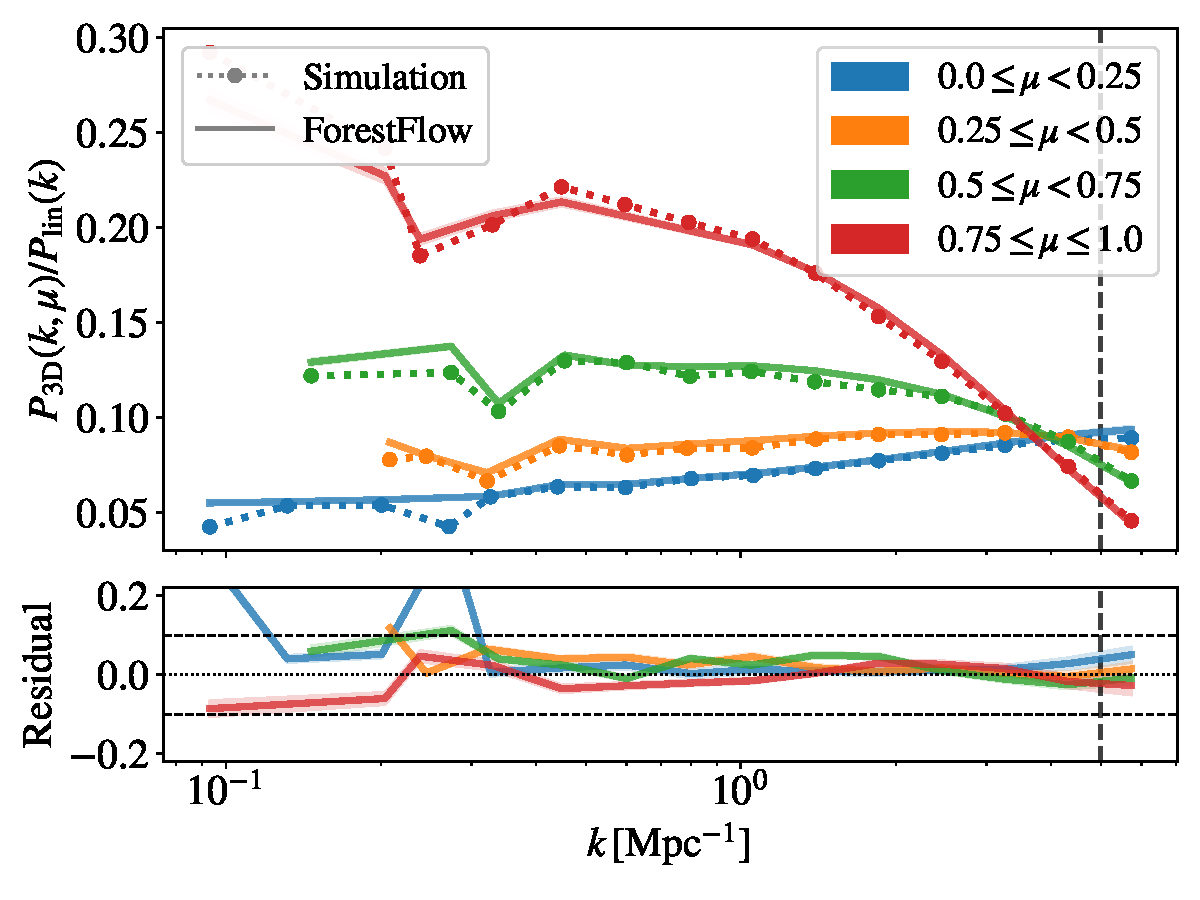
\includegraphics[width= 0.95\columnwidth]{figures/p3d_snap.pdf}
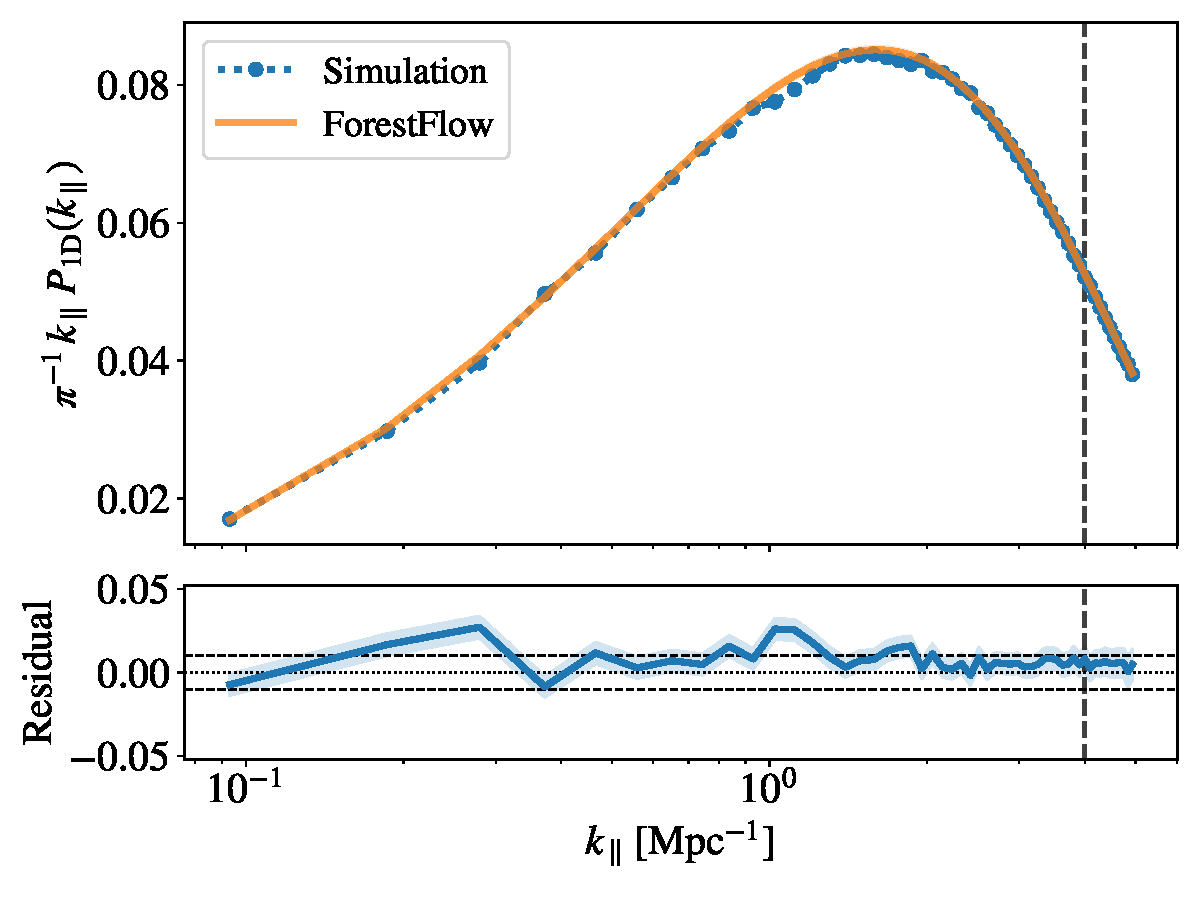
\includegraphics[width= 0.97\columnwidth]{figures/p1d_snap.pdf}
\centering
\caption{Precision of the emulator in recovering \pthreed and \poned measurements from the \simcentral simulation at $z=3$. Dotted lines show measurements from simulations, solid lines and shaded areas display the average and 68\% credible interval of \forestflow predictions, respectively, and vertical dashed lines indicate the minimum scales considered for computing the training data of the emulator. The overall precision of the emulator in recovering \pthreed is 2.0\% on scales not strongly affected by cosmic variance and 0.6\% for \poned.
}
\label{fig:test_snap}
\end{figure}
%%%%%%%%%%%%%%%%%%%

%%%%%%%%%%%%%%%%%%%
\begin{figure*}
\centering
\Large{Leave-simulation-out}\par\medskip
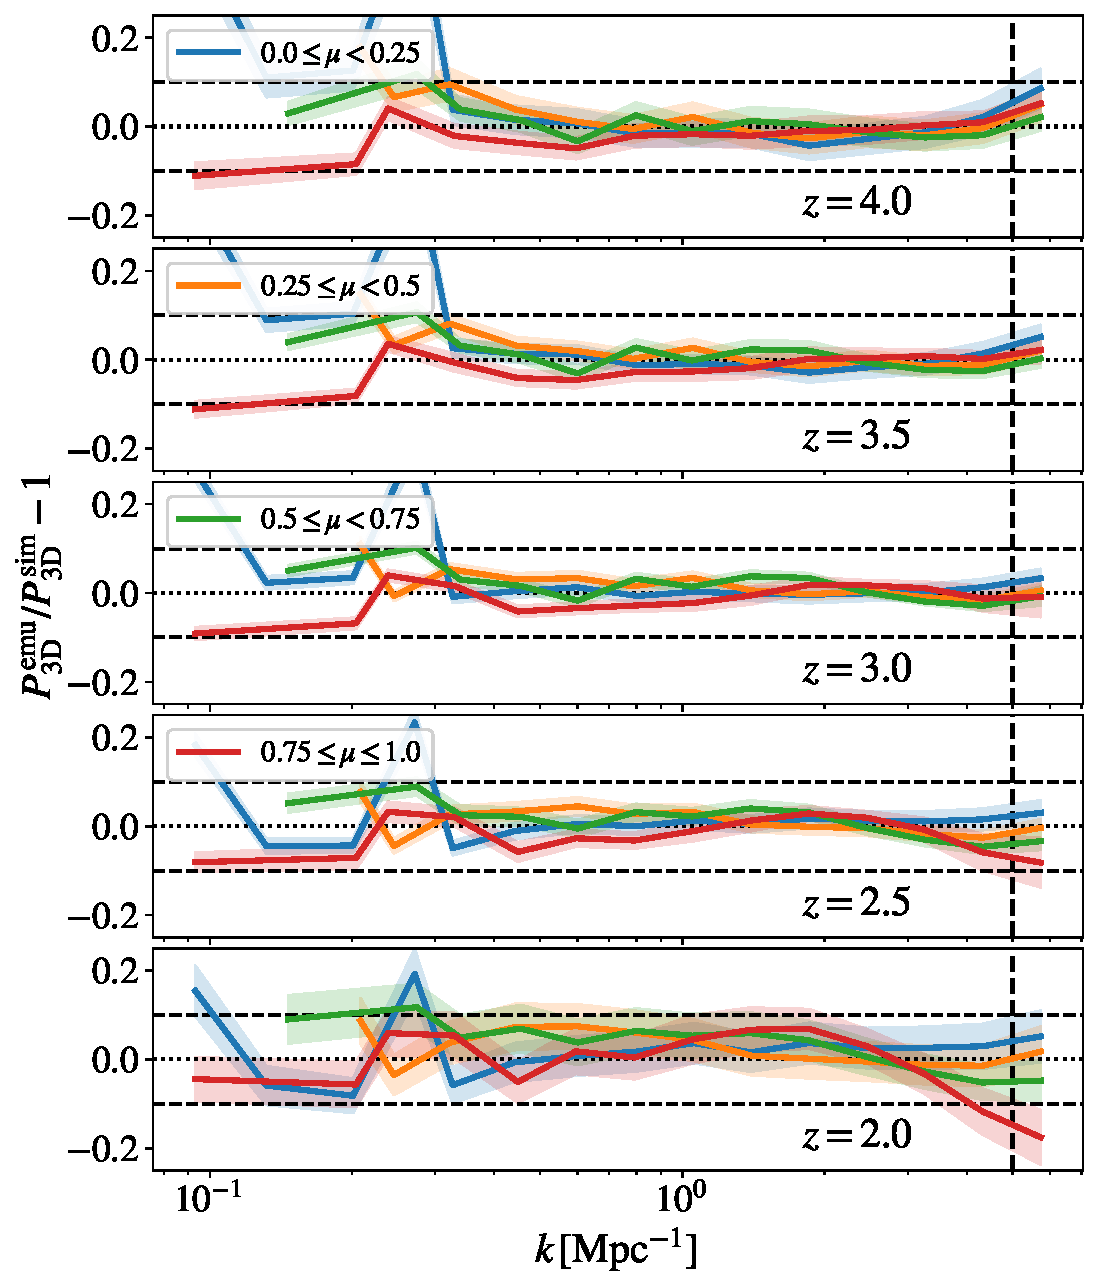
\includegraphics[width= 0.95\columnwidth]{figures/l1O_P3D.pdf}
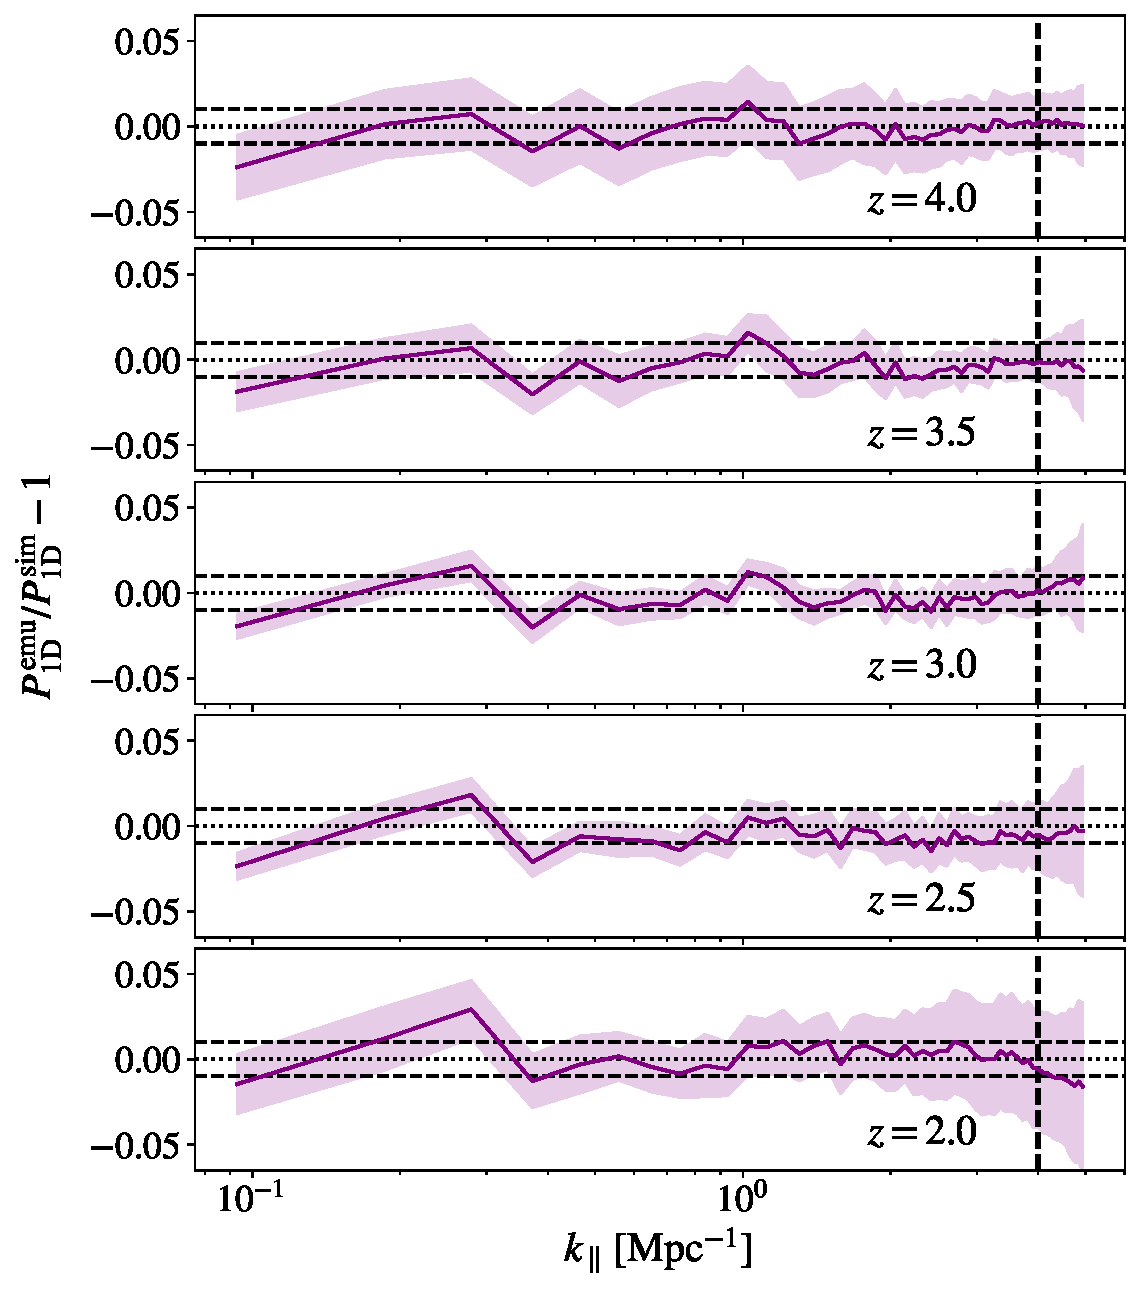
\includegraphics[width= 0.98\columnwidth]{figures/l1O_P1D.pdf}
\Large{Leave-redshift-out}\par\medskip
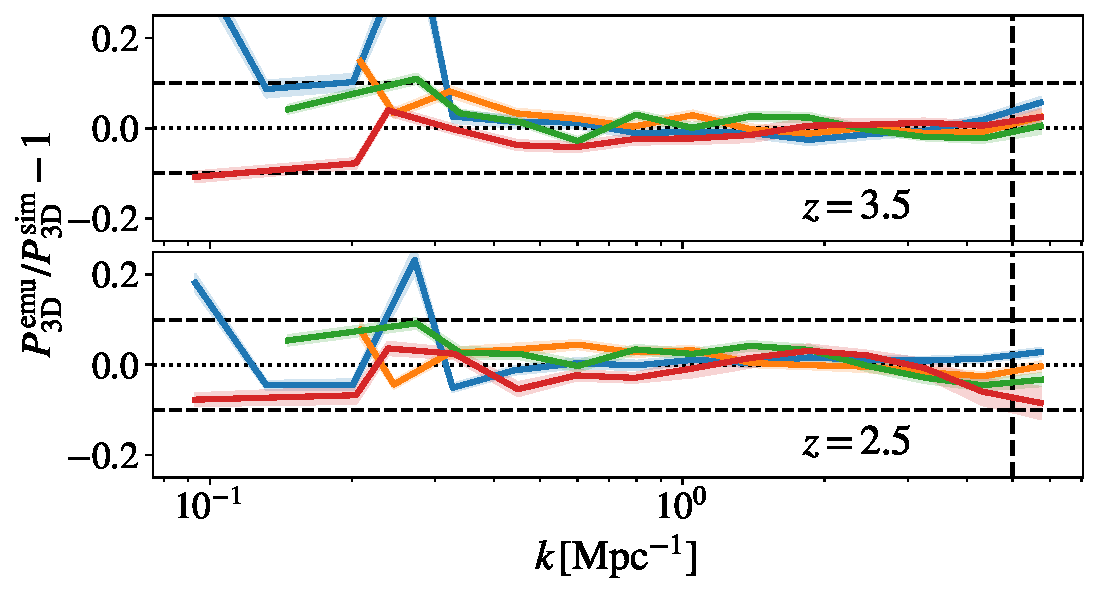
\includegraphics[width= 0.95\columnwidth]{figures/l1O_z_P3D.pdf}
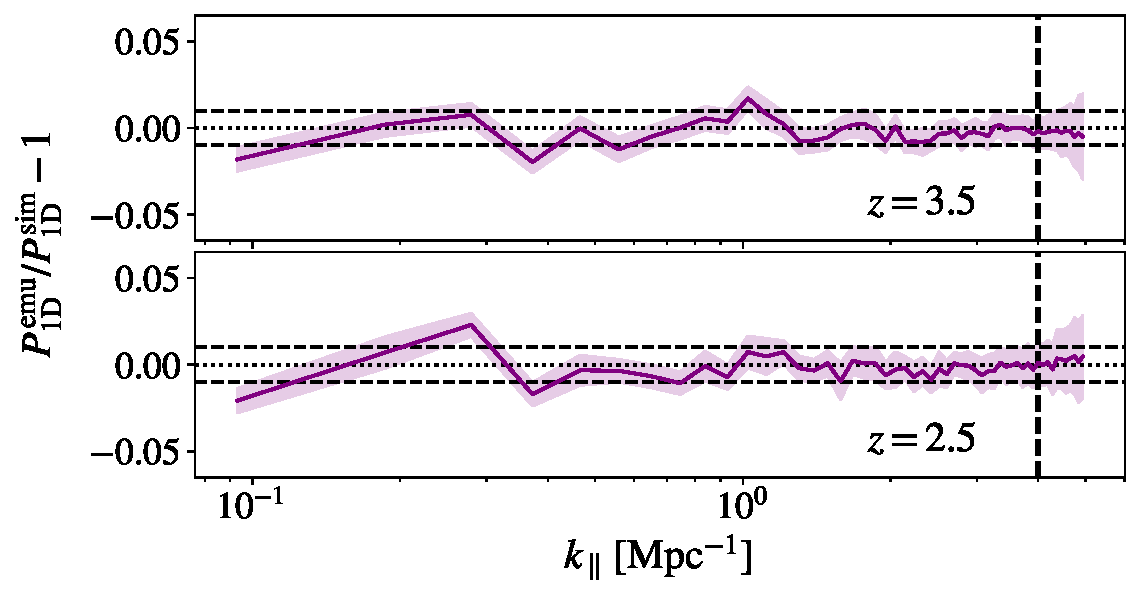
\includegraphics[width= 0.96\columnwidth]{figures/l1O_z_P1D.pdf}
\caption{Precision of the emulator across the input parameter space estimated via leave-simulation-out (top panels) and leave-redshift-out tests (bottom panels). {\bf Top panels.} Each leave-simulation-out test involves training 1 independent emulator with measurements from 29 distinct simulations, and then using the measurements from the remaining simulation as the validation set. Lines and shaded areas show the average and standard deviation of 30 leave-simulation-out tests, and each panel shows the results for a different redshift. {\bf Bottom panels.} Leave-redshift-out tests require optimizing 1 emulator with all measurements but the ones at a particular redshift, and then using measurements from this redshift as validation. Each panel shows the results of a different test.
}
\label{fig:leave_sim_out}
\end{figure*}
%%%%%%%%%%%%%%%%%%%

In this section, we evaluate the precision of \forestflow in recovering the 2 Lyman-$\alpha$ linear biases, which determine the behavior of \pthreed on linear scales, as well as \pthreed and \poned measurements from simulations on the intervals $0.5<k[\iMpc]<5$ and $0.09<k_\parallel[\iMpc]<4$, respectively. These are the ranges of scales used when fitting the parametric model in \S\ref{sec:input} that are not strongly affected by cosmic variance (see \S\ref{sec:strategy_model}). We begin by assessing the precision at the center of the training set, where machine-learning methods typically perform best, and then extend our evaluation across the entire input parameter space.

In Fig.~\ref{fig:test_snap}, we compare measurements of \pthreed and \poned from the \simcentral simulation at $z=3$ with \forestflow predictions. Dotted lines show simulation measurements, while solid lines and shaded areas display the average and 68\% credible interval of \forestflow predictions, respectively. We characterize the accuracy of the credible intervals in Appendix~\ref{sec:uncertainty_validation}. \DIFdelbegin \DIFdel{The overall precision of the emulator in recovering }\DIFdelend \DIFaddbegin \DIFadd{As we can see, the emulator captures the amplitude and scale-dependence of }\DIFaddend \pthreed and \poned \DIFdelbegin \DIFdel{is 2.0 and 0.6\%, respectively. Note that cosmic variance hinders our ability to test the precision of the model; however, this does not necessarily indicate a decrease in model precision for }%DIFDELCMD < \pthreed %%%
\DIFdel{on scales larger than $k=0.5\iMpc$. }%DIFDELCMD < 

%DIFDELCMD < %%%
\DIFdelend \DIFaddbegin \DIFadd{precisely. }\DIFaddend To better characterize the emulator's performance, we compute the average precision of \forestflow in recovering measurements from \simcentral across redshift. We find that it is 1.2 and 0.3\% for $b_\delta$ and $b_\eta$, respectively, which translates into 1.1 and 1.2\% for perpendicular and parallel \pthreed modes on linear scales, and 2.6 and 0.8\% for \pthreed and \poned. \DIFdelbegin \DIFdel{As discussed in \S\ref{sec:input_precision}, }\DIFdelend \DIFaddbegin \DIFadd{Note that cosmic variance hinders our ability to test }\DIFaddend the precision of the \DIFdelbegin \DIFdel{parametric modelin describing }\DIFdelend \DIFaddbegin \DIFadd{model; however, this does not necessarily indicate a decrease in model precision for }\DIFaddend \pthreed \DIFdelbegin \DIFdel{and }%DIFDELCMD < \poned %%%
\DIFdel{measurements is 2.4 and 0.6\%, respectively. Therefore, the primary factor limiting the performance of the emulator at the center of the parameter space is the quality of the training data, and its precision would increase by using bigger simulations with the same resolution to generate the training data}\DIFdelend \DIFaddbegin \DIFadd{on scales larger than $k=0.5\iMpc$}\DIFaddend .

We expect the emulator's efficiency to decrease away from the center of the input space. Ideally, we would have multiple test simulations covering the entire input space to evaluate the performance, but such simulations are unavailable. Instead, we conduct leave-one-out tests, which are widely used to assess the precision of an emulator when the number of training points is insufficient for out-of-sample tests \citep[e.g.;][]{hastie01statisticallearning}. In a leave-one-out test, we optimize \forestflow after removing a subsample from the training set; for example, all measurements from one of the \lacehc simulations. We then check the precision of the new emulator using the subsample held back. By repeating this process for other subsamples, we can estimate the performance of \forestflow across the parameter space. Since each emulator is trained without using the entire dataset, leave-one-out tests provide a lower bound on emulator performance. Additionally, leave-one-out tests may require extrapolating the emulator's predictions, and it is widely known that machine-learning methods do not extrapolate well.

In the top panels of Fig.~\ref{fig:leave_sim_out}, lines and shaded areas display the average and standard deviation of 30 leave-simulation-out tests. Each test requires optimizing an emulator with 29 distinct \lacehc simulations, and then using the remaining simulation as the validation. Each panel shows the results for a different redshift, and we check that the results are similar for redshifts not shown. As we can see, the large-scale noise is similar for all \lacehc simulations; this is because they use the same initial distribution of Fourier phases. The \DIFaddbegin \DIFadd{overall }\DIFaddend performance of \forestflow in recovering $b_\delta$ and $b_\eta$ is 1.0 and 3.1\%, respectively, which translates into 2.0 and 2.9\% for perpendicular and parallel \pthreed modes on linear scales, and 3.4 and 1.8\% for \pthreed and \poned.
\DIFdelbegin \DIFdel{Consequently, the efficiency }\DIFdelend \DIFaddbegin 

%DIF > %%%%%%%%%%%%%%%%%%
\begin{table}
    \caption{\DIFaddFL{Percent precision of the }\pthreed \DIFaddFL{model (Eqs.~\ref{eq:p3d_model} and \ref{eq:dnl}) and }\forestflow \DIFaddFL{in recovering }\pthreed \DIFaddFL{and }\poned\DIFaddFL{, as well as the impact of cosmic variance on these statistics. The second and third columns show the results for }\pthreed \DIFaddFL{and }\poned \DIFaddFL{over the intervals $0.5<k[\iMpc]<5$ and $0.09<k_\parallel[\iMpc]<4$ intervals, respectively, while the last two columns do so for the perpendicular and parallel modes of }\pthreed \DIFaddFL{on linear scales.}}
    \centering
    \begin{tabular}{c|cc|cc|cc}
         \DIFaddFL{Type }& \pthreed & \poned & \DIFaddFL{$b_\delta$ }& \DIFaddFL{$b_\eta$ }& \DIFaddFL{$P_\mathrm{3D, \perp}^\mathrm{lin}$ }& \DIFaddFL{$P_\mathrm{3D, \parallel}^\mathrm{lin}$}\\ \hline
         \DIFaddFL{Cvar. fit}\tablefootmark{a}   & \DIFaddFL{0.8 }& \DIFaddFL{0.1 }& \DIFaddFL{0.6 }& \DIFaddFL{1.8 }& \DIFaddFL{1.2 }& \DIFaddFL{1.8 }\\
         \DIFaddFL{Cvar. data}\tablefootmark{b}  & \DIFaddFL{1.3 }& \DIFaddFL{0.5 }&  \DIFaddFL{-- }&  \DIFaddFL{-- }&   \DIFaddFL{-- }&  \DIFaddFL{-- }\\
         \DIFaddFL{Cvar. \& model}\tablefootmark{c} & \DIFaddFL{2.4 }& \DIFaddFL{0.6 }&  \DIFaddFL{-- }&   \DIFaddFL{-- }&   \DIFaddFL{-- }&   \DIFaddFL{-- }\\
         \DIFaddFL{Emu. center}\tablefootmark{d}  & \DIFaddFL{2.6 }& \DIFaddFL{0.8 }& \DIFaddFL{1.2 }& \DIFaddFL{0.3 }& \DIFaddFL{1.1 }& \DIFaddFL{1.2 }\\
         \DIFaddFL{Emu. overall}\tablefootmark{e} & \DIFaddFL{3.4 }& \DIFaddFL{1.8 }& \DIFaddFL{1.0 }& \DIFaddFL{3.1 }& \DIFaddFL{2.0 }& \DIFaddFL{2.9 }\\
    \end{tabular}
    \tablefoot{
        \tablefoottext{a}{Impact of cosmic variance on the best-fitting fitting \pthreed model to simulation measurements (see Appendix~\ref{sec:cosmic_variance}).}
        \tablefoottext{b}{Impact of cosmic variance on simulation measurements (see Appendix~\ref{sec:cosmic_variance}).}
        \tablefoottext{c}{Joint impact of cosmic variance and the limited flexibility of the \pthreed model (see \S\ref{sec:input_precision}).}
        \tablefoottext{d}{Precision of \forestflow at the center of the parameter space, estimated using the \simcentral simulation (see \S\ref{sec:results_statistics}).}
        \tablefoottext{e}{Precision of \forestflow across the parameter space, estimated via leave-simulation-out tests (see \S\ref{sec:results_statistics}).}
    }
    \label{tab:precision}
\end{table}
%DIF > %%%%%%%%%%%%%%%%%%

\DIFadd{In Table~\ref{tab:precision}, we gather the precision of }\forestflow \DIFadd{at the center and }\DIFaddend across the parameter space\DIFdelbegin \DIFdel{is approximately 2 times worse than at the center for the 2 }%DIFDELCMD < \lya %%%
\DIFdel{linear biases }\DIFdelend \DIFaddbegin \DIFadd{, as well as the expected level of uncertainties due to cosmic variance and the limited flexibility of the }\pthreed \DIFadd{model. Given that we use our simulations to evaluate the precision of }\forestflow\DIFadd{, and the impact of cosmic variance on simulation measurements is 1.3 and 0.5\% on }\pthreed \DIFaddend and \poned\DIFdelbegin \DIFdel{, while it is 31\% worse }\DIFdelend \DIFaddbegin \DIFadd{, respectively, these numbers limits the maximum precision we can test with our simulations. These levels would decrease by evaluating the precision using bigger simulations with the same resolution. Uncertainties due to the impact of cosmic variance on the training data and inaccuracies of the }\pthreed \DIFadd{model in describing }\pthreed \DIFadd{and }\poned \DIFadd{are 2.4 and 0.6\% for these statistics, respectively, which is 1.1 and 0.1\% worse than the impact of cosmic variance on simulation measurements. At the center of the parameter space, the precision of }\forestflow \DIFaddend for \pthreed \DIFdelbegin \DIFdel{. These numbers }\DIFdelend \DIFaddbegin \DIFadd{and }\poned \DIFadd{is only 0.2\% worse than the previous levels, letting us conclude that the primary factors limiting the performance of }\forestflow \DIFadd{at the center of the parameter space are the size of the training simulations and model inaccuracies. 
}

\DIFadd{The efficiency of }\forestflow \DIFadd{across the parameter space is 1.2 and 1.0\% worse than at the center for }\pthreed \DIFadd{and }\poned\DIFadd{, respectively. Consequently, the precision of the emulator }\DIFaddend would likely improve by increasing the number of training simulations\DIFdelbegin \DIFdel{; nevertheless, the precision estimated via }\DIFdelend \DIFaddbegin \DIFadd{. However, }\DIFaddend leave-one-out tests \DIFdelbegin \DIFdel{is always worse than at the center }\DIFdelend \DIFaddbegin \DIFadd{significantly underestimate the precision at the edges }\DIFaddend of the training set\DIFaddbegin \DIFadd{, especially }\DIFaddend for a small number of simulations\DIFaddbegin \DIFadd{, }\DIFaddend because it often requires extrapolating the emulator's predictions. \DIFdelbegin %DIFDELCMD < 

%DIFDELCMD < %%%
\DIFdel{By considering the results at the center and across the parameter space, we conclude that the size and number of }\DIFdelend \DIFaddbegin \DIFadd{We can thus conclude that the quality of the training data, }\DIFaddend the \DIFdelbegin %DIFDELCMD < \lacehc %%%
\DIFdelend \DIFaddbegin \DIFadd{precision of the model, and the number of training }\DIFaddend simulations have a similar impact on the performance of \forestflow. Given that \DIFdelbegin \DIFdel{leave-one-out tests only }\DIFdelend \DIFaddbegin \DIFadd{leave-simulation-out tests tend }\DIFaddend provide a lower bound for the emulator's performance, we conclude that the \DIFaddbegin \DIFadd{overall }\DIFaddend precision of \forestflow in predicting \pthreed from linear scales to $k=5\iMpc$ is approximately 3\%, and $\simeq1.5\%$ for \poned down to $k_\parallel=4\iMpc$.

As discussed in \S\ref{sec:strategy_params}, \forestflow uses as input parameters measured from each snapshot of the training simulations rather than "traditional" cosmological parameters such as $\Omega_m$, $A_s$, or $H_0$. This strategy enables training \forestflow without specifying the input redshift and making predictions for redshifts not present in the training set. To test this assumption, we carry out two leave-redshift-out tests. The first involves optimizing one emulator with all \lacehc measurements but the ones at $z=2.5$, and then validating it with data from this redshift. For the second, we follow the same approach but using measurements at $z=3.5$. We display the results of these tests in the bottom panels of Fig.~\ref{fig:leave_sim_out}. The precision of the emulator is similar for leave-redshift-out and leave-simulation-out tests, validating the approach mentioned above. We find similar results for leave-redshift-out tests at other redshifts.

%%%%%%%%%%%%%%%%%%%
%%%%%%%%%%%%%%%%%%%

%%%%%%%%%%%%%%%%%%%
\begin{figure*}
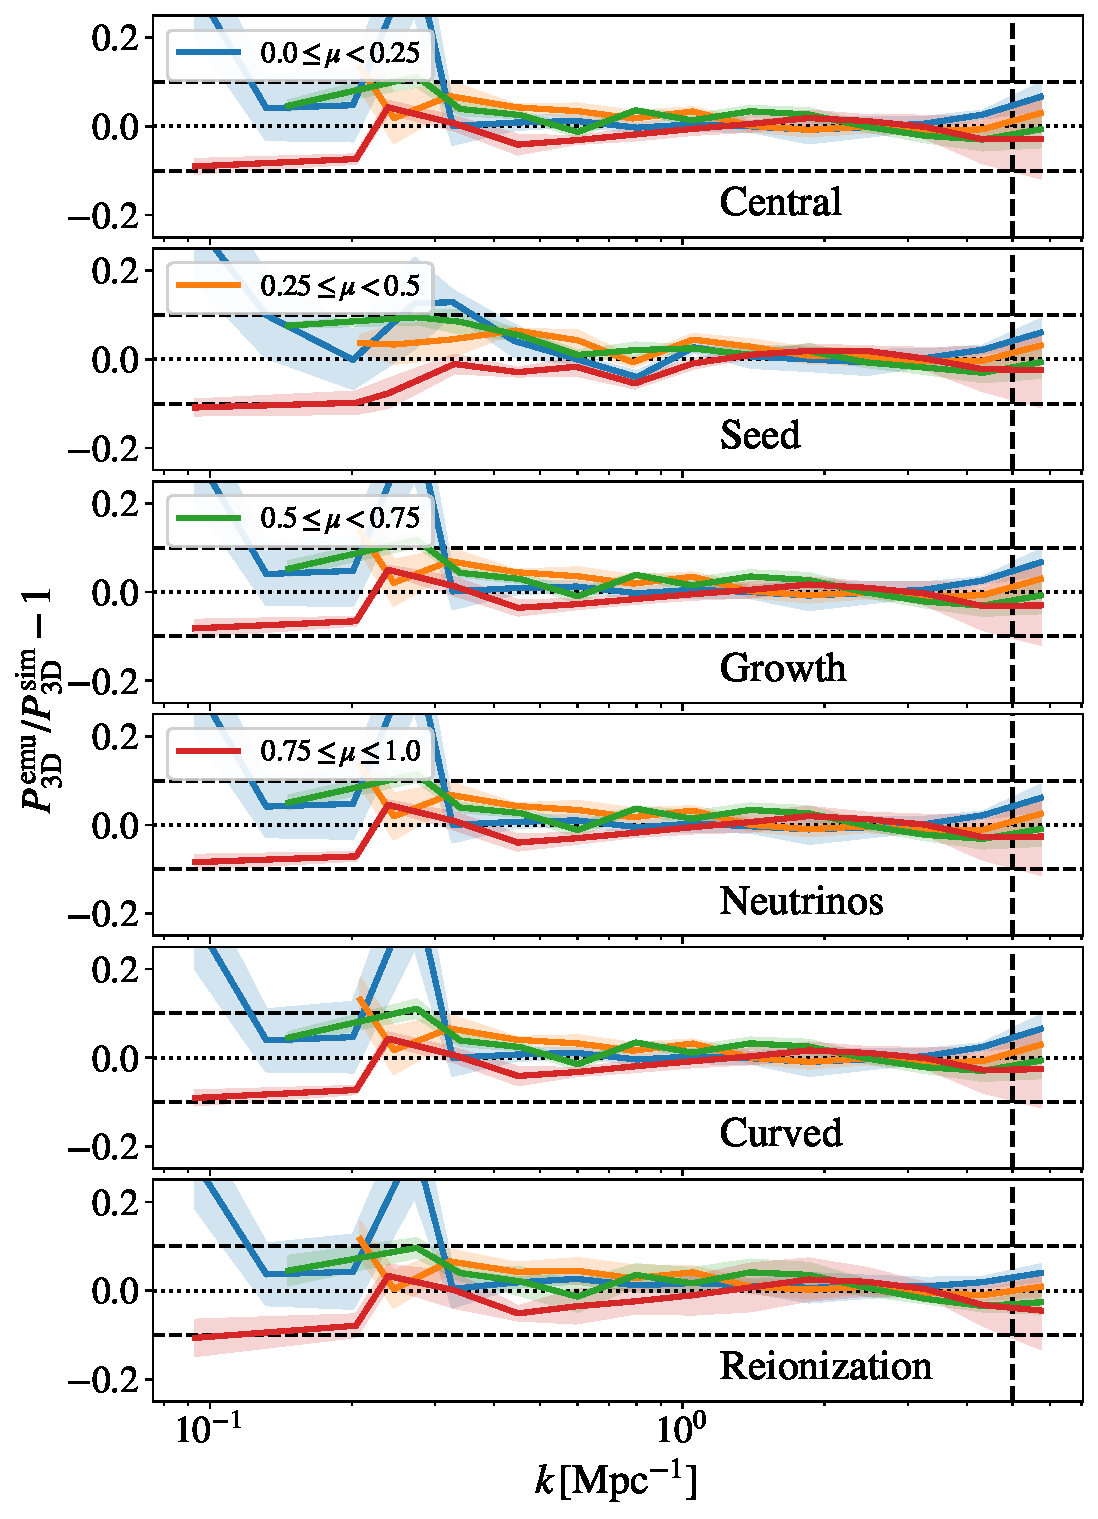
\includegraphics[width= 0.95\columnwidth]{figures/test_cosmo_P3D.pdf}
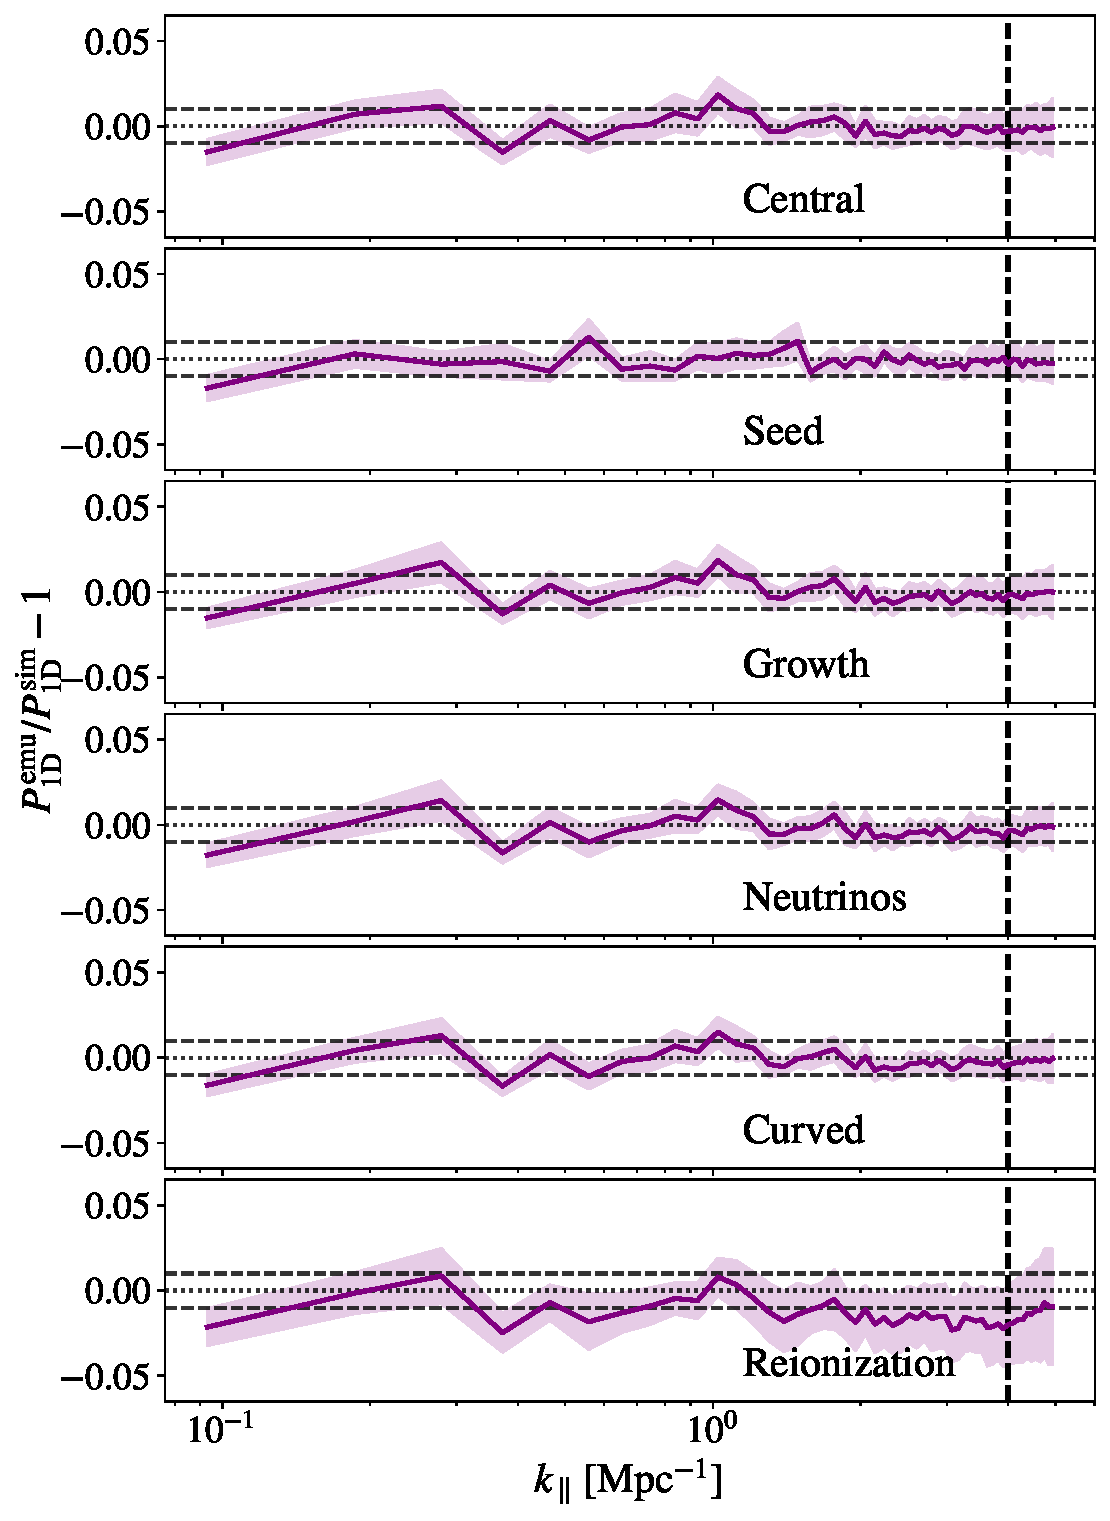
\includegraphics[width= 0.96\columnwidth]{figures/test_cosmo_P1D.pdf}
\centering
\caption{Precision of the emulator in recovering \pthreed and \poned for test simulations not included in the training set. Lines and shaded areas display the average and standard deviation of the results for 11 snapshots between $z=2$ and 4.5, respectively. From top to bottom, the rows show the results for the \simcentral, \simseed, \simh, \simnu, \simcurved, and \simigm simulations, where the \simcentral and \simseed simulations are at the center of the input parameter space and employ the same and different initial distribution of Fourier phases as the training simulations, respectively, the \simh and \simigm simulations use a different growth and reionization history relative to those used by the \lacehc simulations, and the \simnu and \simcurved simulations consider massive neutrinos and curvature. The efficiency of \forestflow is approximately the same for all simulations.}
\label{fig:other_cosmo}
\end{figure*}
%%%%%%%%%%%%%%%%%%%


\subsection{\DIFdelbegin \DIFdel{Test simulations}\DIFdelend \DIFaddbegin \DIFadd{Cosmologies and IGM histories outside the training set}\DIFaddend }
\label{sec:results_other}

In Fig.~\ref{fig:other_cosmo}, we examine the precision of \forestflow reproducing \pthreed and \poned measurements from simulations \DIFdelbegin \DIFdel{outside }\DIFdelend \DIFaddbegin \DIFadd{not included in }\DIFaddend the training set. Lines indicate the redshift average of the relative difference between model predictions and simulation measurements. The first two rows show the results for the \simcentral and \simseed simulations, whose only difference is their initial distribution of phases. Consequently, the predictions of \forestflow are the same for both. As we can see, these simulations present a different large-scale pattern of fluctuations, signaling that are caused by cosmic variance. Once we ignore these, we find that the precision of \forestflow is practically the same for both simulations. We can thus conclude that \forestflow predictions are largely insensitive to the impact of cosmic variance on the training set.

In the third, fourth, and fifth rows of Fig.~\ref{fig:other_cosmo}, we use the \simh, \simnu, and \simcurved simulations to evaluate the precision of \forestflow for three different scenarios not contemplated in the training set: different growth history, massive neutrinos, and curvature. As we can see, the precision of \forestflow for all these simulations is approximately the same as for the \simcentral simulation. These results support that using the small-scale amplitude and slope of the linear power spectrum to capture cosmological information enables setting precise constraints on growth histories and $\Lambda$CDM extensions not included in the training set \citep[see also][]{Pedersen2021, pedersen2023CompressingCosmologicalInformation, cabayol-garcia2023NeuralNetworkEmulator}.

In the last row of Fig.~\ref{fig:other_cosmo}, we examine the precision of \forestflow for the \simigm simulation, which employs a \ion{He}{ii} reionization history significantly different from those used by the \lacehc simulations. The precision of the emulator for this and the \simcentral simulation is similar, which is noteworthy given that the performance of \poned emulators for the \simigm is significantly worse than for the \simcentral simulation \citep{cabayol-garcia2023NeuralNetworkEmulator}. The outstanding performance of \forestflow is likely because the relationship between IGM physics and the parameters of the \pthreed model is more straightforward than with \poned variations.


%%%%%%%%%%%%%%%%
%%%%%%%%%%%%%%%%
%%%%%%%%%%%%%%%%

\section{Discussion}
\label{sec:discussion}

Cosmological analyses of the \lya forest come in two flavors: one-dimensional studies focused on small, non-linear scales and three-dimensional analyses of large, linear scales. With \forestflow, we can now consistently model \lya correlations from nonlinear to linear scales, enabling a variety of promising analyses that we discuss next.

%%%%%%%%%%%%%%%%
%%%%%%%%%%%%%%%%

\subsection{Connecting large-scale biases with small-scale physics}
\label{sec:discussion_large_small}

%DIF > %%%%%%%%%%%%%%%%%%
\DIFaddbegin \begin{figure*}
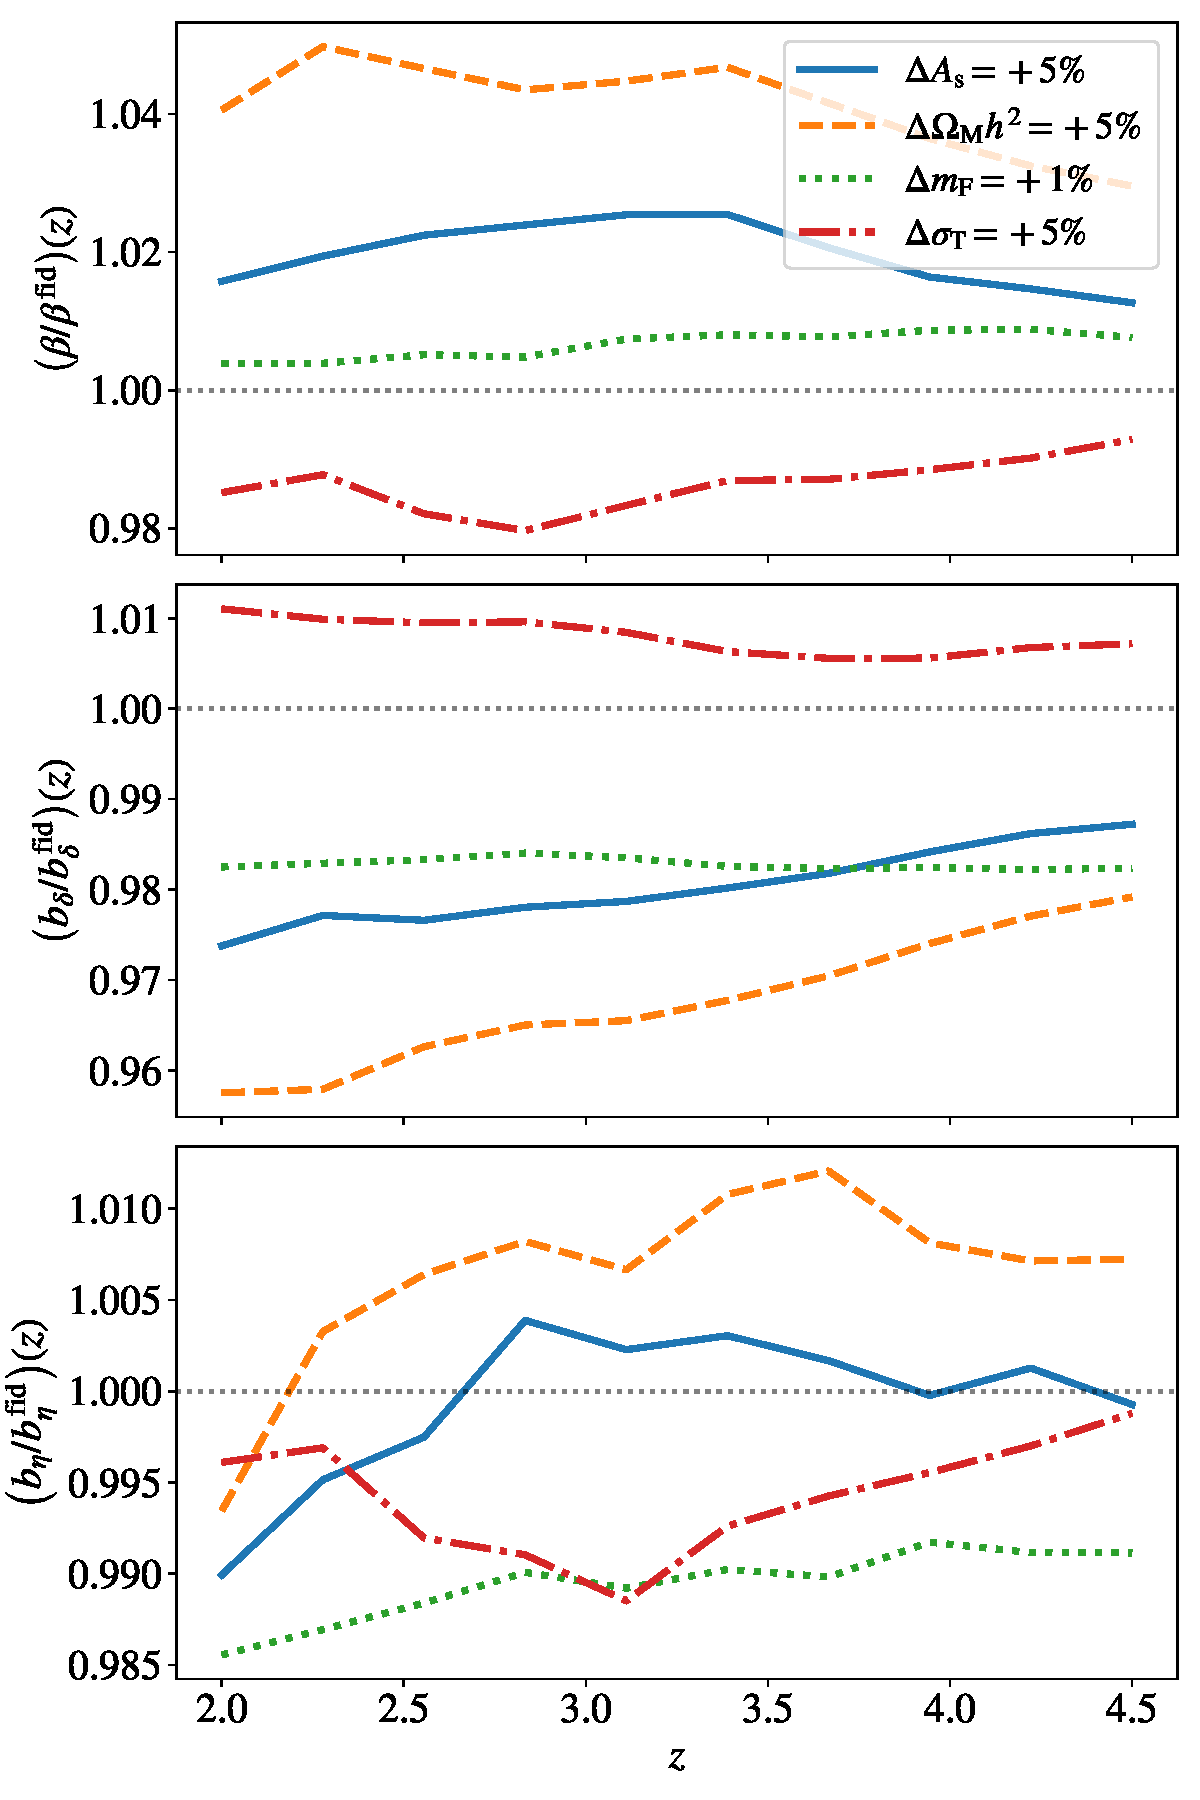
\includegraphics[width=\columnwidth]{figures/sensitivity_lbias.pdf}
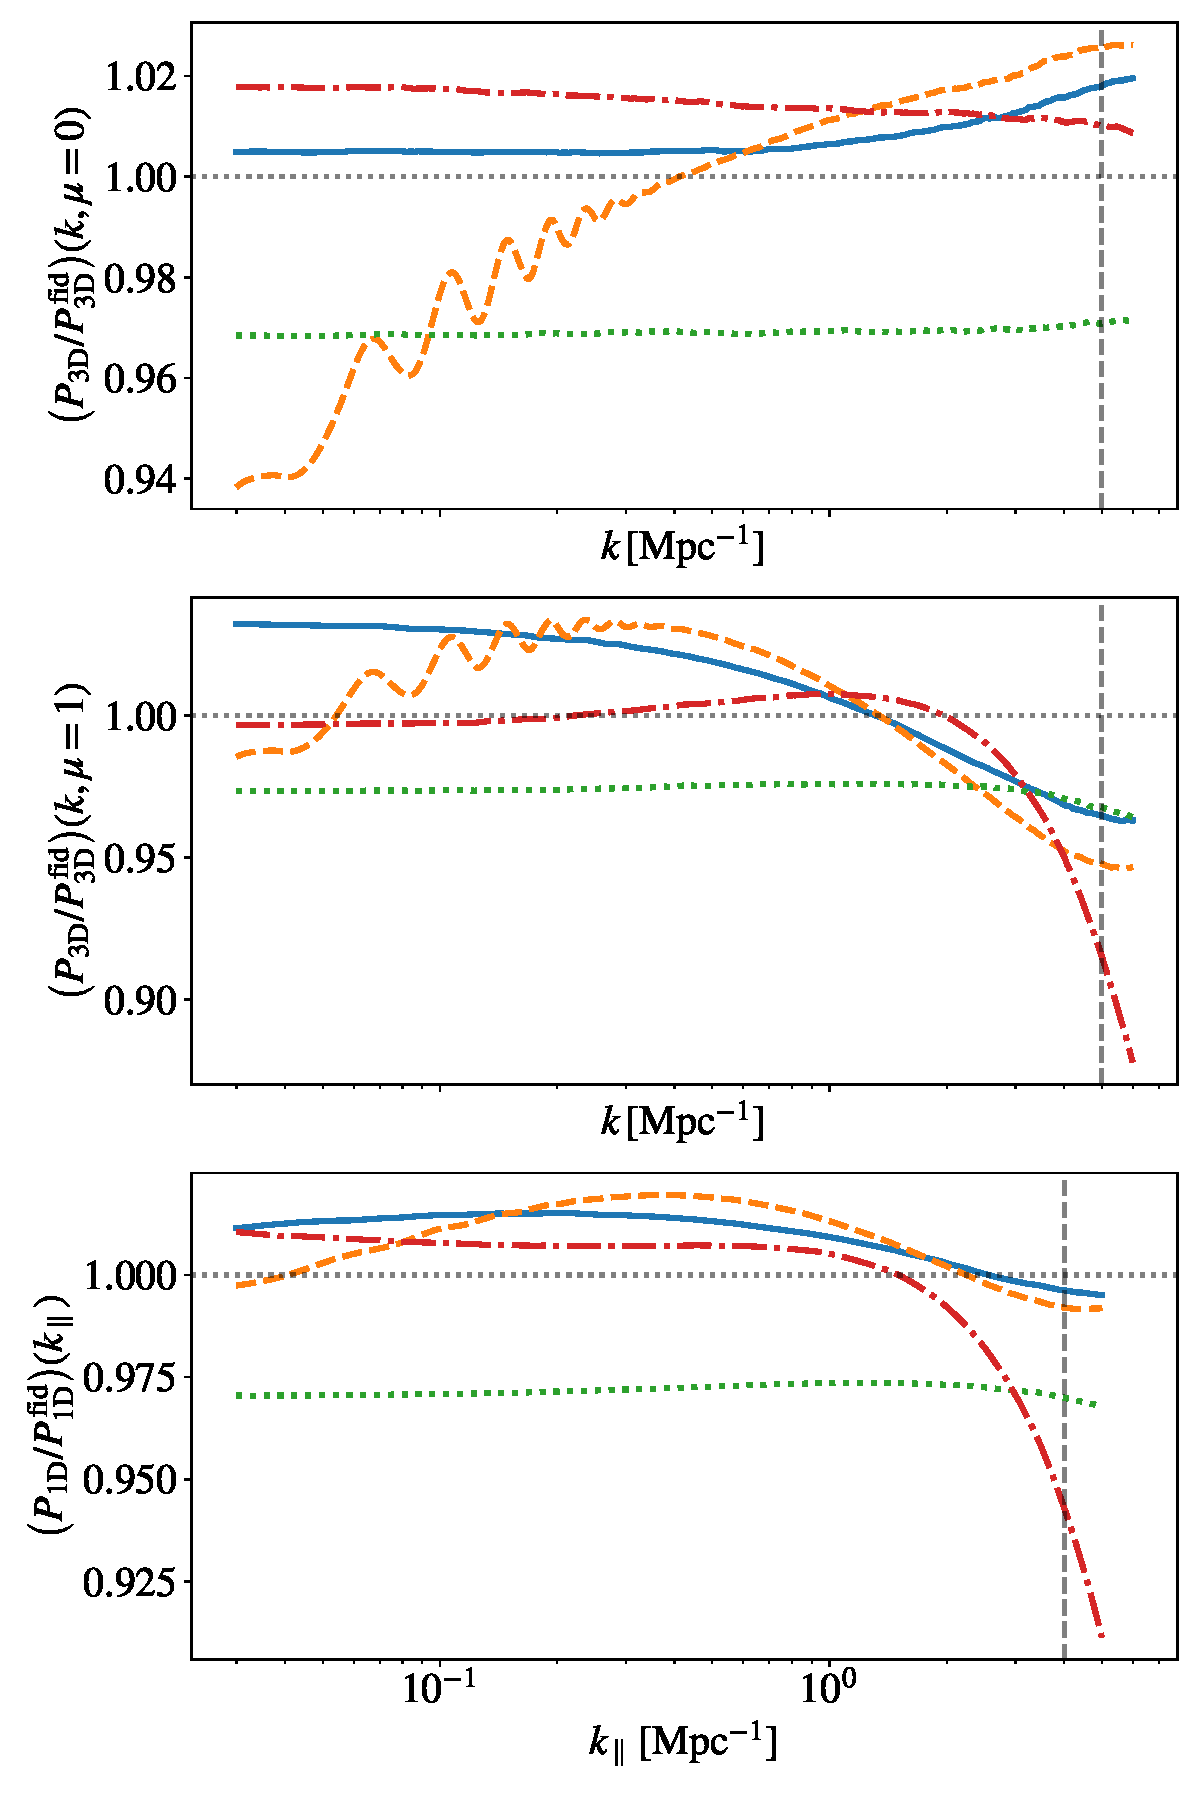
\includegraphics[width=\columnwidth]{figures/sensitivity_power.pdf}
\centering
\caption{\DIFaddFL{Response of }\lya \DIFaddFL{clustering to variations in cosmology and IGM physics according to }\forestflow\DIFaddFL{. The top, middle, and bottom panels of the left column show the results for $\beta$, $b_\delta$, and $b_\eta$, respectively, while those of the right column do so for the perpendicular modes of }\pthreed\DIFaddFL{, the parallel modes of }\pthreed\DIFaddFL{, and }\poned\DIFaddFL{. Blue, orange, and red lines show the response of the previous quantities to a 5\% increase in $A_\mathrm{s}$, $\Omega_\mathrm{M}h^2$, and $\sigma_\mathrm{T}$, respectively, while green lines do so for a 1\% increase in $\bar{F}$.
}}
\label{fig:sensitivity}
\end{figure*}
%DIF > %%%%%%%%%%%%%%%%%%

\DIFaddend Small-scale \lya analyses use emulators to predict \poned as a function of cosmology and IGM physics \DIFdelbegin \DIFdel{\mbox{%DIFAUXCMD
\citep[e.g.;][]{Pedersen2021, pedersen2023CompressingCosmologicalInformation, cabayol-garcia2023NeuralNetworkEmulator}}\hspace{0pt}%DIFAUXCMD
}\DIFdelend \DIFaddbegin \DIFadd{\mbox{%DIFAUXCMD
\citep[e.g.;][]{ cabayol-garcia2023NeuralNetworkEmulator}}\hspace{0pt}%DIFAUXCMD
}\DIFaddend , while large-scale analyses use linear or perturbation theory models to predict \xithreed together with \lya linear bias parameters that need to be marginalized over. \forestflow provides a relationship between IGM physics and linear biases, enabling the use of \poned studies to inform three-dimensional analyses and vice versa.

We could use \forestflow to \DIFdelbegin \DIFdel{fit }%DIFDELCMD < \poned %%%
\DIFdel{measurements to }\DIFdelend set constraints on $b_\delta$ and $b_\eta$ \DIFaddbegin \DIFadd{by fitting }\poned \DIFadd{measurements, }\DIFaddend and then use these \DIFaddbegin \DIFadd{constraints }\DIFaddend as priors in three-dimensional studies\DIFdelbegin \DIFdel{, breaking degeneracies between large-scale }\DIFdelend \DIFaddbegin \DIFadd{. As a result, we would break degeneracies between }\lya \DIFadd{linear }\DIFaddend bias parameters and cosmology\DIFdelbegin \DIFdel{. As a result, we could }\DIFdelend \DIFaddbegin \DIFadd{, allowing us to }\DIFaddend measure the amplitude of linear density and velocity fluctuations, $\sigma_8(z)$ and $f \sigma_8(z)$\DIFaddbegin \DIFadd{, }\DIFaddend rather than $b_\delta \sigma_8$ and $b_\eta f \sigma_8$ like in traditional \lyaf analyses. \DIFdelbegin \DIFdel{Similarly, we could use measurements of linear bias parameters from three-dimensional analyses \mbox{%DIFAUXCMD
\citep{dumasdesbourboux2020CompletedSDSSIVExtended, 2024arXiv240403001D} }\hspace{0pt}%DIFAUXCMD
to make predictions for IGM parameters, which could be used as priors in }%DIFDELCMD < \poned %%%
\DIFdel{studies.
}%DIFDELCMD < 

%DIFDELCMD < %%%
\DIFdelend To illustrate this application, we \DIFdelbegin \DIFdel{compare }%DIFDELCMD < \forestflow %%%
\DIFdel{predictions for }\DIFdelend \DIFaddbegin \DIFadd{proceed to compare measurements of }\DIFaddend $b_\delta$ and \DIFdelbegin \DIFdel{$\beta$ with measurements from observations}\DIFdelend \DIFaddbegin \DIFadd{$\beta\equiv b_\delta^{-1} b_\eta f$ from BAO analyses with }\forestflow \DIFadd{predictions based }\poned \DIFadd{analyses}\DIFaddend . The analysis of BAO in the \lyaf from the first data release of DESI yields $b_\delta=-0.108\pm0.005$ and $\beta=1.74\pm0.09$ at $z=2.33$ \citep{desicollaboration2024DESI2024IV}. \DIFaddbegin \DIFadd{On the other hand, }\DIFaddend \forestflow predicts $b_\delta=-0.118$ and $\beta=1.57$ \DIFaddbegin \DIFadd{at $z=2.33$ }\DIFaddend for a {\it Planck} cosmology \DIFdelbegin \DIFdel{at the same redshift when using }\DIFdelend \DIFaddbegin \DIFadd{when using as input }\DIFaddend the best-fitting constraints on IGM parameters from table 4 of \citet{emugp_Walther2019}, which were derived from high-resolution \poned measurements. Even though the constraints on IGM parameters were derived using a \poned emulator trained on simulations with possibly slightly different definitions of \DIFdelbegin \DIFdel{the IGM parameters }\DIFdelend \DIFaddbegin \DIFadd{IGM parameters relative to those used in this work}\DIFaddend , \forestflow predictions and DESI measurements agree at the 2 sigma level, encouraging this new type of study.

\DIFaddbegin \DIFadd{In the left panels of Fig.~\ref{fig:sensitivity}, we display }\forestflow \DIFadd{predictions for the response of the }\lya \DIFadd{linear biases and $\beta$ to variations in cosmology and IGM physics. The response of $b_\delta$ to these changes is strong and have a different redshift dependence for cosmology and IGM parameters; therefore, we could use }\forestflow \DIFadd{to analyze }\pthreed \DIFadd{measurements from different redshifts to further break degeneracies between $b_\delta$ and $\sigma_8$. On the other hand, the response of $b_\eta$ to these changes is weak, and it is thus challenging to use this approach to break degeneracies between $b_\eta$ and $f \sigma_8$. Note that the response of the }\lya \DIFadd{linear biases and $\beta$ to $A_\mathrm{s}$ variations broadly agrees with measurements from simulations run while only varying $\sigma_8$ \mbox{%DIFAUXCMD
\citep{arinyo-i-prats2015NonlinearPowerSpectrum}}\hspace{0pt}%DIFAUXCMD
.
}

\DIFadd{Similarly, we could use measurements of linear bias parameters from three-dimensional analyses \mbox{%DIFAUXCMD
\citep{dumasdesbourboux2020CompletedSDSSIVExtended, desicollaboration2024DESI2024IV} }\hspace{0pt}%DIFAUXCMD
to make predictions for IGM parameters, which could be used in }\poned \DIFadd{studies to break degeneracies between cosmology and IGM physics. In the right panels of Fig.~\ref{fig:sensitivity}, we display }\forestflow \DIFadd{predictions for the response of }\pthreed \DIFadd{and }\poned \DIFadd{to variations in cosmology and IGM physics. As we can see, the response of }\poned \DIFadd{to $A_\mathrm{s}$ and $\bar{F}$ variations is largely scale-independent down to $k_\parallel=1\iMpc$ where many other effects are at play, and thus these two parameters are largely degenerated. On the other hand, this is not the case for }\pthreed\DIFadd{; consequently, we could use information from }\pthreed \DIFadd{analyses to break degeneracies in }\poned \DIFadd{studies. Note that the response of }\pthreed \DIFadd{and }\poned \DIFadd{to $A_\mathrm{s}$, $\bar{F}$, and $\sigma_\mathrm{T}$ variations broadly agrees with measurements from simulations run varying only one of these parameters at a time \mbox{%DIFAUXCMD
\citep{mcdonald2003MeasurementCosmologicalGeometry, mcdonald2005LinearTheoryPower}}\hspace{0pt}%DIFAUXCMD
.
}

\DIFadd{We also observe that }\pthreed \DIFadd{and }\poned \DIFadd{response significantly to variations in $\Omega_\mathrm{M}h^2$, suggesting that the }\lya \DIFadd{clustering is highly sensitive the expansion and growth history. However, we find that variations in $A_\mathrm{s}$ and $n_\mathrm{s}$ can absorb the changes in }\pthreed \DIFadd{and }\poned \DIFadd{to the 2\% level, and completely do so for }\pthreed \DIFadd{at the pivot scale of the cosmological parameters of }\forestflow\DIFadd{, $k_\mathrm{p}=0.7\iMpc$. Furthermore, }{\it \DIFadd{Planck}} \DIFadd{measured $\Omega_\mathrm{M}h^2$ with 0.8\% precision \mbox{%DIFAUXCMD
\citet{planckcollaboration2020Planck2018Resultsa}}\hspace{0pt}%DIFAUXCMD
, and $A_\mathrm{s}$ and $n_\mathrm{s}$ absorb 1\% variations in $\Omega_\mathrm{M}h^2$ to the $\simeq0.4\%$ level. This result supports the approach of not considering any cosmological parameter related to variations in the expansion of growth history as input for }\forestflow \DIFadd{(see also \S\ref{sec:results_other}).
}


\DIFaddend %%%%%%%%%%%%%%%%
%%%%%%%%%%%%%%%%

\subsection{Alcock-Paczy\'nski on mildly non-linear scales}

Thanks to the increasing precision of galaxy surveys, there is a growing interest in extracting cosmological information from increasingly smaller scales in three-dimensional analyses. An avenue to do so is to analyze anisotropies in the correlation function \citet[AP test;][]{alcock1979EvolutionFreeTesta}, first proposed in the context of the \lyaf by \citet{1999ApJ...518...24M, hui1999GeometricalTestCosmological}. Recently, \cite{cuceu2023ConstraintsCosmicExpansion} followed this approach to analyze \lyaf measurements from the Sloan Digital Sky Survey (SDSS) data release 16 \citep[DR16;][]{Ahumada2020_DR16}, yielding constraints on some cosmological parameters a factor of two tighter than those from BAO-only analyses. 

This study modeled three-dimensional correlations using linear theory, which restricted the range of scales analyzed to those larger than $25 \hMpc$. We could significantly extend the range of scales used in this type of analysis by modeling three-dimensional correlations using \forestflow. As a result, the constraining power of AP analyses would be much larger. Furthermore, we could use \forestflow to extract information from \poned analyses to reduce degeneracies between cosmology and the parameters describing \xithreed (see \S\ref{sec:discussion_large_small}).

%%%%%%%%%%%%%%%%
%%%%%%%%%%%%%%%%

\subsection{Extending 3D analyses to the smallest scales}

%%%%%%%%%%%%%%%%
\begin{figure}
    \centering
    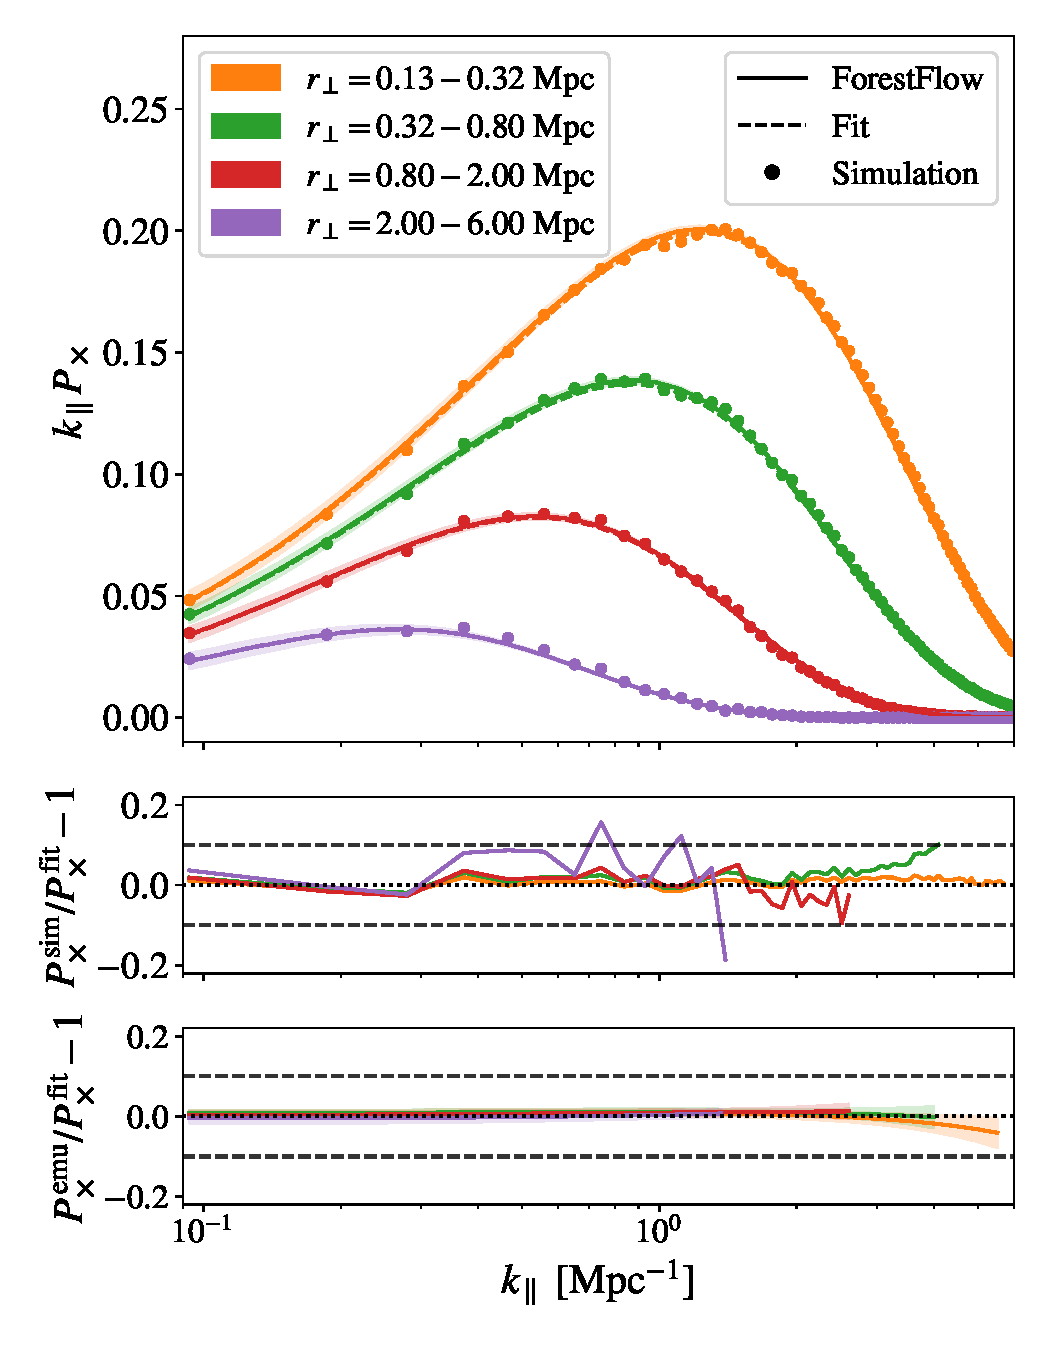
\includegraphics[width=.9\columnwidth]{figures/Pcross_central_snap6_kPx_allbin_emupred_first4_withfracerr.pdf}
    \caption{Precision of the parametric model and the emulator in describing \pcross measurements from the \simcentral simulation at $z=3$. Dots show simulation measurements, dashed lines depict predictions from the best-fitting parametric model to \pthreed and \poned measurements, and solid lines and shaded areas display the average and 68\% credible interval of \forestflow predictions. The color of the lines indicates the results for different bins in transverse separation $r_\perp$. The middle panel shows the residual between simulation measurements and \DIFdelbeginFL \DIFdelFL{the best-fitting }\DIFdelendFL model \DIFaddbeginFL \DIFaddFL{predictions}\DIFaddendFL , while the bottom panel displays the residual between \DIFdelbeginFL \DIFdelFL{the best-fitting }\DIFdelendFL model and emulator predictions. The precision of \forestflow in reproducing simulation measurements is \DIFdelbeginFL \DIFdelFL{approximately the same as }\DIFdelendFL \DIFaddbeginFL \DIFaddFL{similar to that of }\DIFaddendFL the best-fitting model.}
    \label{fig:Px_onesnap}
\end{figure}
%%%%%%%%%%%%%%%%


The ultimate goal of \forestflow is to perform a joint analysis of one- and three-dimensional measurements from small to large scales. An interesting approach to do so is to measure the \lyaf cross-spectrum \citep[\pcross; e.g.;][]{hui1999GeometricalTestCosmological, fontribera2018HowEstimate3D}, which captures the correlation between one-dimensional Fourier modes from two neighboring quasars separated by a transverse separation ($r_\perp$). We can model this statistic by taking the inverse Fourier transform of \pthreed only along the perpendicular directions
%
\begin{align}
    P_{\times}(k_{\parallel}, r_\perp) &\equiv \frac{1}{(2\pi)^2}\int \mathrm{d}\boldsymbol{k}_\perp \, e^{i\,\boldsymbol{k}_\perp\cdot \boldsymbol{r}_\perp} \, P_\mathrm{3D}(k_\parallel, k_\perp) \nonumber\\ 
    &= \frac{1}{2\pi} \int_0^{\infty}  \mathrm{d}k_\perp\,  k_\perp\, J_0 (k_\perp r_\perp) \, P_\mathrm{3D}(k_\parallel, k_\perp) ~. \label{eq:pcross_bessel}
\end{align}
%
Comparing this equation with Eq.~\ref{eq:p1d}, it becomes clear that \poned is a special case of \pcross, corresponding to the limit where the transverse separation is zero.

In \S\ref{sec:input_fitting}, we optimize the \pthreed model to describe measurements of \pthreed and \poned from the \lacehc simulations. Then, in \S\ref{sec:forestflow}, we use the distribution of best-fitting parameters as the training set for \forestflow, which predicts the value of \pthreed model parameters as a function of cosmology and IGM physics. Even though neither the best-fitting model nor \forestflow use \pcross for their optimization, we can make predictions of \pcross for both. To do so, we first estimate \pthreed using the value of the model parameters using Eq.~\ref{eq:p3d_model}, and then we integrate it using Eq.~\ref{eq:pcross_bessel}. We carry out the integration using the fast Hankel transform algorithm \texttt{FFTlog} \citep{Hamilton2000MNRAS.312..257H} implemented in the \texttt{hankl} package \citep{karamanis2021hankl}.

We use \pcross measurements from the simulations described in \S~\ref{sec:input_sims} to evaluate the precision of \forestflow for this statistic. We first define four bins in $r_\perp$, the transverse separation between skewers in configuration space, with edges 0.13, 0.32, 0.80, 2, and 6 Mpc. Then, we measure \pcross using all pairs of skewers with $r_\perp$ separation within the previous bins 
%
\begin{equation}
    P_\times(r_\perp, k_\parallel) = \bigg \langle \Re \Big[\tilde{\delta_\mathrm{i}}(k_\parallel) \tilde{\delta_\mathrm{j}}^*(k_\parallel)\Big]\bigg\rangle \,
\end{equation}
%
where $\tilde{\delta}_\mathrm{i}$ and $\tilde{\delta}^*_\mathrm{j}$ stand for the Fourier transform of a skewer $i$ and the complex conjugate of its partner $j$, respectively, the average $\langle\rangle$ includes all possible pairs in the bin without repetition or permutation, and $\Re$ indicates that we only use the real part of the expression between brackets because the average of the imaginary part is zero. The $r_\perp$ on the left-hand side denotes the effective center of the bin, accounting for the skewed distribution of $r_\perp$ within each bin: the number of skewers separated by a small distance $\mathrm{d}r_\perp$ is proportional to $r_\perp$, and therefore the effective center is not at the halfway point. To compute \pcross at the effective center, we perform the integration using ten sub-bins within each $r_\perp$ bin and calculate the average of these weighted by $r_\perp$.

In Fig.~\ref{fig:Px_onesnap}, we \DIFdelbegin \DIFdel{compare measurements of }\DIFdelend \DIFaddbegin \DIFadd{study the precision of }\forestflow \DIFadd{in reproducing }\DIFaddend \pcross \DIFaddbegin \DIFadd{measurements }\DIFaddend from the \simcentral simulation at $z=3$\DIFdelbegin \DIFdel{with }\DIFdelend \DIFaddbegin \DIFadd{. Dots display simulation measurements, dashed lines }\DIFaddend the best-fitting model to \pthreed and \poned measurements from this simulation\DIFdelbegin \DIFdel{and }\DIFdelend \DIFaddbegin \DIFadd{, and the solid lines }\DIFaddend \forestflow predictions. As we can see, \pcross decreases as the $r_\perp$ separation increases; this is because more distant sightlines are sampling increasingly uncorrelated regions. In the middle panel, we examine the precision of the best-fitting model in describing \DIFdelbegin \DIFdel{the data}\DIFdelend \DIFaddbegin \DIFadd{simulation measurements}\DIFaddend , finding that it is better than 10\% throughout all the scales shown. The \DIFaddbegin \DIFadd{precision of the model improves for smaller $r_\perp$ separations. This is likely because the fit's likelihood function (Eq.~\ref{eq:chi2}) considers }\poned\DIFadd{, which is equivalent to }\pcross \DIFadd{at $r_\perp=0$ separation, but not }\pcross\DIFadd{. The }\DIFaddend bottom panel addresses the performance of \forestflow relative to the best-fitting model\DIFdelbegin \DIFdel{so we can evaluate the precision }\DIFdelend \DIFaddbegin \DIFadd{; in this way, we approximately evaluate the performance }\DIFaddend of the emulator in \DIFdelbegin \DIFdel{the absence of cosmic variance. As we can see, the precision of the emulator }\DIFdelend \DIFaddbegin \DIFadd{reproducing the training data. The precision of }\forestflow \DIFaddend in recovering the best-fitting model is better than 5\% for all scales \DIFaddbegin \DIFadd{shown}\DIFaddend .

Future studies could use \forestflow for extracting constraints on cosmology and IGM physics from the analysis of \pcross measurements \citep[e.g.;][]{Karim2023}. Nevertheless, as with \poned, these analyses would also require modeling multiple systematics affecting \lya measurements such as damped \lya systems, metal line contamination, and AGN feedback.


%%%%%%%%%%%%%%%%
%%%%%%%%%%%%%%%%
%%%%%%%%%%%%%%%%

\section{Conclusions}
\label{sec:conclusions}

We present \forestflow, a cosmological emulator that predicts \lya clustering from linear to nonlinear scales. Using an architecture based on conditional normalizing flows, \forestflow emulates the 2 linear \lya biases \DIFaddbegin \DIFadd{($b_\delta$ and $b_\eta$) }\DIFaddend and 6 physically-motivated parameters capturing small-scale deviations of the three-dimensional flux power spectrum (\pthreed) from linear theory. We summarize the main results of this work below:

\begin{itemize}
    \item The main advantage of our strategy, compared to emulating \pthreed at a set of $k$-bins, is that \forestflow can predict \lya clustering on arbitrarily large (linear) scales when combined with a Boltzmann solver. Additionally, the emulator can make predictions for any statistics derived from \pthreed without interpolation or extrapolation, including the two-point correlation function (\xithreed, main statistic of large-scale studies), the one-dimensional \lya flux power spectrum (\poned, main statistic of small-scale studies), and the cross-spectrum (\pcross, promising statistic for full-scale studies).

    \item To train the emulator, we use the best-fitting value of the 8 model parameters to \pthreed and \poned measurements from a suite of 30 fixed-and-paired cosmological hydrodynamical simulations spanning 11 equally-spaced redshifts between $z=2$ and 4.5. We emulate these parameters as a function of the small-scale amplitude and slope of the linear power spectrum, the mean transmitted flux fraction, the amplitude and slope of the temperature-density relation, and the pressure smoothing scale \citep[see][]{Pedersen2021}. We use this parameterization because it has the potential for making predictions for extensions to the $\Lambda$CDM model and ionization histories not included in the training set \citep[][]{ pedersen2023CompressingCosmologicalInformation, cabayol-garcia2023NeuralNetworkEmulator}. 

    \item In \S\ref{sec:results_statistics}, we show that the precision of \textsc{forestflow} in predicting $P_\mathrm{3D}$ from linear scales to $k=5\iMpc$ is 3\% and 1.5\% for $P_\mathrm{1D}$ down to $k_\parallel=4\iMpc$. \DIFdelbegin \DIFdel{Interestingly, }\DIFdelend \DIFaddbegin \DIFadd{We find that }\DIFaddend the size and number of training simulations have a similar impact on the emulator's performance \DIFdelbegin \DIFdel{, while }\DIFdelend \DIFaddbegin \DIFadd{as }\DIFaddend uncertainties arising from the limited flexibility of the 8-parameter model\DIFdelbegin \DIFdel{are subdominant}\DIFdelend . 

    \item In \S\ref{sec:results_other}, we show that \forestflow displays similar performance as before for two extensions to the $\Lambda$CDM model --- massive neutrinos and curvature --- and ionization histories not included in the training set. 
\end{itemize}

The release of \forestflow is timely for \lyaf analyses with the ongoing Dark Energy Spectroscopic Instrument (DESI) survey. As noted in \S\ref{sec:discussion}, \forestflow enables a series of novel multiscale studies with DESI data, including connecting large- and small-scale analyses as well as extending three-dimensional analyses towards smaller scales.


%%%%%%%%%%%%%%%%
%%%%%%%%%%%%%%%%
%%%%%%%%%%%%%%%%

\begin{acknowledgements}
JCM, LCG, ML, and AFR acknowledge support from the European Union’s Horizon Europe research and innovation programme (COSMO-LYA, grant agreement 101044612). AFR acknowledges financial support from the Spanish Ministry of Science and Innovation under the Ramon y Cajal program (RYC-2018-025210) and the PGC2021-123012NB-C41 project. IFAE is partially funded by the CERCA program of the Generalitat de Catalunya. The analysis has been performed at Port d’Informaci\'o Cient\'ifica (PIC); we acknowledge the support provided by PIC in granting us access to their computing resources.

This material is based upon work supported by the U.S. Department of Energy (DOE), Office of Science, Office of High-Energy Physics, under Contract No. DE–AC02–05CH11231, and by the National Energy Research Scientific Computing Center, a DOE Office of Science User Facility under the same contract. Additional support for DESI was provided by the U.S. National Science Foundation (NSF), Division of Astronomical Sciences under Contract No. AST-0950945 to the NSF’s National Optical-Infrared Astronomy Research Laboratory; the Science and Technology Facilities Council of the United Kingdom; the Gordon and Betty Moore Foundation; the Heising-Simons Foundation; the French Alternative Energies and Atomic Energy Commission (CEA); the National Council of Humanities, Science and Technology of Mexico (CONAHCYT); the Ministry of Science and Innovation of Spain (MICINN), and by the DESI Member Institutions: \url{https://www.desi.lbl.gov/collaborating-institutions}. Any opinions, findings, and conclusions or recommendations expressed in this material are those of the author(s) and do not necessarily reflect the views of the U. S. National Science Foundation, the U. S. Department of Energy, or any of the listed funding agencies. The authors are honored to be permitted to conduct scientific research on Iolkam Du’ag (Kitt Peak), a mountain with particular significance to the Tohono O’odham Nation.
\end{acknowledgements}

%%%%%%%%%%%%%%%%%%%%%%%%%%%%%%%%%%%%%%%%%%%%%%%%%%
\section*{Data Availability}

\forestflow and all the notebooks used to generate the plots of this paper can be found in \url{https://github.com/igmhub/ForestFlow}, as well as all data points shown in the published graphs. The simulations utilized for training and testing the emulator are publicly accessible at \url{https://github.com/igmhub/LaCE}.


%%%%%%%%%%%%%%%%%%%% REFERENCES %%%%%%%%%%%%%%%%%%

% The best way to enter references is to use BibTeX:

\bibliographystyle{aa_url}
\bibliography{forestflow} % if your bibtex file is called example.bib

\begin{appendix}

%%%%%%%%%%%%%%%%%%%
%%%%%%%%%%%%%%%%%%%

\section{Cosmic variance}
\label{sec:cosmic_variance}

%%%%%%%%%%%%%%%%%%%
\begin{figure}
    \centering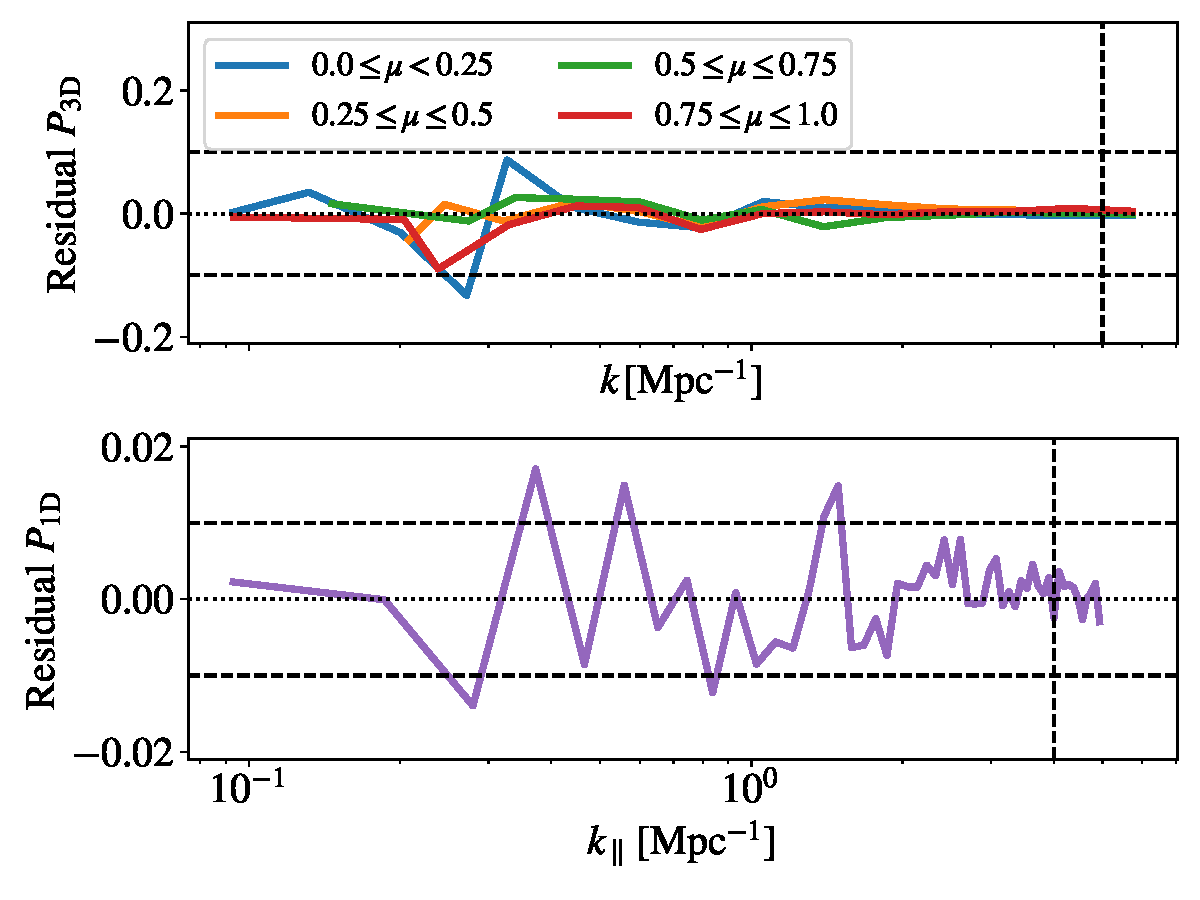
\includegraphics[width=\columnwidth]{figures/cvariance_z_3.0.pdf}
    \caption{Impact of cosmic variance on \DIFdelbeginFL \DIFdelFL{measurements of }\DIFdelendFL \pthreed (top panel) and \poned (bottom panel) \DIFaddbeginFL \DIFaddFL{measurements }\DIFaddendFL from our simulations at $z=3$. \DIFdelbeginFL \DIFdelFL{Solid and dashed lines }\DIFdelendFL \DIFaddbeginFL \DIFaddFL{Lines }\DIFaddendFL show the difference between measurements from \DIFaddbeginFL \DIFaddFL{the }\DIFaddendFL \simcentral and \simseed \DIFaddbeginFL \DIFaddFL{simulations, which only differ on their initial distribution of Fourier phases, }\DIFaddendFL divided by $\sqrt{2}$ times their average. \DIFdelbeginFL \DIFdelFL{We use the same color coding as in the main body. }\DIFdelendFL Cosmic variance induces errors as large as 10\% on \pthreed for $k\simeq0.3\iMpc$, while these are of the order of $1\%$ for \poned.}
    \label{fig:cvar}
\end{figure}
%%%%%%%%%%%%%%%%%%%


%%%%%%%%%%%%%%%%%%%
\begin{figure}
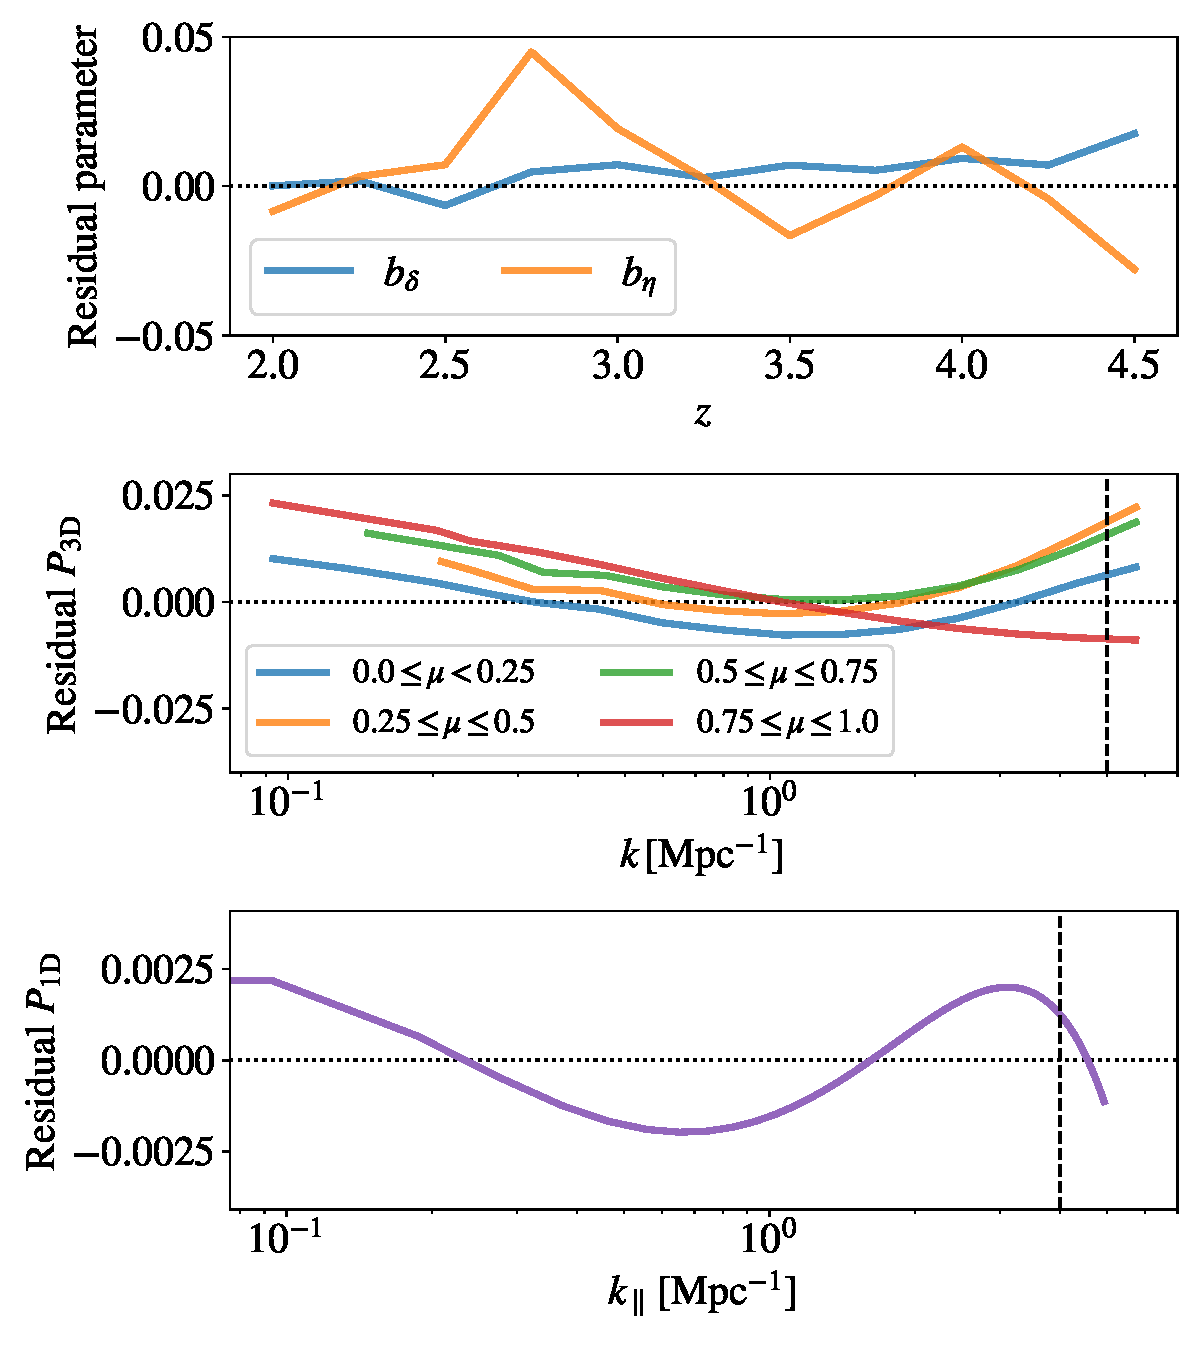
\includegraphics[width=\columnwidth]{figures/cvar_fit_z_3.0.pdf}
\centering
\caption{Impact of cosmic variance on predictions from the \pthreed parametric model. Lines show the difference between the best-fitting \DIFdelbeginFL \DIFdelFL{model }\DIFdelendFL \DIFaddbeginFL \DIFaddFL{models }\DIFaddendFL to \DIFaddbeginFL \pthreed \DIFaddFL{and }\poned \DIFaddFL{measurements from }\DIFaddendFL the \simcentral and \simseed simulations, \DIFdelbeginFL \DIFdelFL{which only differ on their initial distribution of Fourier phases, }\DIFdelendFL divided by $\sqrt{2}$ times the best-fitting model to their average. The top panel shows the results for the \lya linear biases \DIFdelbeginFL \DIFdelFL{, which sets }%DIFDELCMD < \pthreed %%%
\DIFdelFL{on linear scales}\DIFdelendFL \DIFaddbeginFL \DIFaddFL{($b_\delta$ and $b_\eta$)}\DIFaddendFL , while the middle and bottom panels display the results for \pthreed and \poned at $z=3$\DIFdelbeginFL \DIFdelFL{across the range of scales used in the fit}\DIFdelendFL \DIFaddbeginFL \DIFaddFL{, respectively}\DIFaddendFL . The impact of cosmic variance on \DIFdelbeginFL \DIFdelFL{$b_\delta$ and $b_\eta$ }\DIFdelendFL \DIFaddbeginFL \DIFaddFL{model predictions }\DIFaddendFL is \DIFdelbeginFL \DIFdelFL{0.6 and 1.8\%, respectively, and 0.8 and 0.1\% for }%DIFDELCMD < \pthreed %%%
\DIFdelFL{and }%DIFDELCMD < \poned %%%
\DIFdelFL{throughout the full range }\DIFdelendFL \DIFaddbeginFL \DIFaddFL{approximately an order }\DIFaddendFL of \DIFdelbeginFL \DIFdelFL{scales shown}\DIFdelendFL \DIFaddbeginFL \DIFaddFL{magnitude smaller than on simulation measurements (see Fig.~\ref{fig:cvar})}\DIFaddendFL .}
\label{fig:cvar_fit}
\end{figure}
%%%%%%%%%%%%%%%%%%%

Throughout this work, we train and test \forestflow using simulations run employing the "fixed-and-paired" technique \citep{angulo2016CosmologicalNbodySimulations, pontzen2016InvertedInitialConditions}, which significantly reduces cosmic variance for the clustering of the \lyaf \citep{anderson2019CosmologicalHydrodynamicSimulations}. \DIFdelbegin \DIFdel{Ideally, we would }\DIFdelend \DIFaddbegin \DIFadd{We could further mitigate the impact of cosmic variance by using control variates \mbox{%DIFAUXCMD
\citep{Kokron2022}}\hspace{0pt}%DIFAUXCMD
, but this is outside the scope of the current work. The impact of cosmic variance on fixed-and-paired simulations is not straightforward \mbox{%DIFAUXCMD
\citep{maion2022fpvariance}}\hspace{0pt}%DIFAUXCMD
, and thus we would ideally }\DIFaddend use multiple fixed-and-paired simulations with different initial distributions of Fourier phases to estimate the precision of \DIFdelbegin \DIFdel{measurements of these statistics from our simulations}\DIFdelend \DIFaddbegin \DIFadd{simulation measurements}\DIFaddend . However, we only have two simulations with these properties: \simcentral and \simseed. In this section, we use these two simulations to estimate the impact of cosmic variance on simulation measurements and best-fitting models.

In Fig.~\ref{fig:cvar}, we display the difference between measurements from the \simcentral and \simseed at $z=3$ divided by $\sqrt{2}$ times their average\DIFdelbegin \DIFdel{. We employ the factor $\sqrt{2}$ to estimate the noise for a single simulation. In simulations with random initial conditions, }\DIFdelend \DIFaddbegin \footnote{\DIFadd{We use the factor $\sqrt{2}$ to estimate the noise for a single simulation.}}\DIFadd{. The }\simcentral \DIFadd{and }\simseed \DIFadd{simulations only differ on their initial distribution of Fourier phases, and thus their difference isolates }\DIFaddend the impact of cosmic variance\DIFdelbegin \DIFdel{on }%DIFDELCMD < \pthreed %%%
\DIFdelend \DIFaddbegin \DIFadd{. In contrast to traditional simulations, where cosmic variance }\DIFaddend is inversely proportional to the square root of the number of modes \DIFdelbegin \DIFdel{, which grows with $k^3$. However, in our fixed-and-paired simulations, errors reach approximately 10\% }\DIFdelend \DIFaddbegin \DIFadd{for }\pthreed\DIFadd{, this source of uncertainty reaches $\simeq10\%$ }\DIFaddend at $k\simeq0.3\iMpc$ and \DIFdelbegin \DIFdel{decrease for }\DIFdelend \DIFaddbegin \DIFadd{decreases at both }\DIFaddend larger and smaller scales. This \DIFdelbegin \DIFdel{is because }\DIFdelend \DIFaddbegin \DIFadd{trend can be explained as follows: the reduction at the largest scales is due to }\DIFaddend the fix-and-paired technique\DIFaddbegin \DIFadd{, which }\DIFaddend completely cancels out cosmic variance for linear density modes\DIFdelbegin \DIFdel{but }\DIFdelend \DIFaddbegin \DIFadd{. Conversely, the increase at intermediate scales is attributed to }\DIFaddend non-linear evolution\DIFdelbegin \DIFdel{(in particular mode coupling) re-introduces it }\DIFdelend \DIFaddbegin \DIFadd{, particularly mode coupling, which reintroduces cosmic variance }\DIFaddend on mildly non-linear scales\DIFdelbegin \DIFdel{\mbox{%DIFAUXCMD
\citep{maion2022fpvariance}}\hspace{0pt}%DIFAUXCMD
. Consequently, this source of error hinders of ability to use our simulations}\DIFdelend \DIFaddbegin \DIFadd{. For even smaller scales, the number of modes increases, leading to a decrease in cosmic variance, similar to what is observed in traditional simulations.
}

\DIFadd{The main consequence of cosmic variance is that it hinders our ability }\DIFaddend to evaluate the precision of \DIFdelbegin \DIFdel{both the }%DIFDELCMD < \pthreed %%%
\DIFdelend \DIFaddbegin \DIFadd{the }\DIFaddend model and the emulator \DIFdelbegin \DIFdel{in \S\ref{sec:input_precision} and \ref{sec:results}, respectively}\DIFdelend \DIFaddbegin \DIFadd{with our simulations}\DIFaddend . To mitigate the impact of \DIFdelbegin \DIFdel{cosmic variance in these tests, we restrict our analysis of }\DIFdelend \DIFaddbegin \DIFadd{this source of uncertainty, we quote the precision of the model and emulator for }\DIFaddend \pthreed \DIFdelbegin \DIFdel{to }\DIFdelend \DIFaddbegin \DIFadd{on }\DIFaddend scales smaller than $k=0.5\iMpc$ \DIFdelbegin \DIFdel{, as these scales are less affected by cosmic variance}\DIFdelend \DIFaddbegin \DIFadd{throughout the main body of the test}\DIFaddend . Conversely, \DIFaddbegin \DIFadd{the impact of cosmic variance on }\DIFaddend \poned \DIFdelbegin \DIFdel{measurements are minimally impacted by cosmic variance across all scales, allowing us to include the largest scales measured in the simulations }\DIFdelend \DIFaddbegin \DIFadd{is approximately 1.5\% at $k_\parallel<2\iMpc$, much smaller than for }\pthreed\DIFadd{, letting us include all scales in the tests }\DIFaddend without concern.

For a more precise estimation\DIFdelbegin \DIFdel{of the impact of cosmic variance on simulation measurements}\DIFdelend , we compute the standard deviation of the \DIFdelbegin \DIFdel{ratios }\DIFdelend \DIFaddbegin \DIFadd{results }\DIFaddend shown in Fig.~\ref{fig:cvar} \DIFdelbegin \DIFdel{using the 11 redshifts for which we have simulation measurements}\DIFdelend \DIFaddbegin \DIFadd{across redshift}\DIFaddend . We do so within the intervals $0.5<k[\iMpc]<5$ and $0.09<k_\parallel[\iMpc]<4$ for \pthreed and \poned, respectively, motivated by the previous discussion and the range of scales used when fitting the \pthreed model in \S\ref{sec:input_fitting}. We find that the average impact of cosmic variance on \pthreed and \poned is 1.3 and 0.5\%, respectively. 
\DIFdelbegin \DIFdel{In what follows, we }\DIFdelend \DIFaddbegin 

\DIFadd{We now proceed to }\DIFaddend study the impact of \DIFdelbegin \DIFdel{this source of uncertainty on predictions from }\DIFdelend \DIFaddbegin \DIFadd{cosmic variance on }\DIFaddend the best-fitting \DIFaddbegin \DIFadd{model for simulation measurements of }\DIFaddend \pthreed \DIFdelbegin \DIFdel{model to simulation measurements , which constitute the training data of }%DIFDELCMD < \forestflow%%%
\DIFdel{. }%DIFDELCMD < 

%DIFDELCMD < %%%
\DIFdelend \DIFaddbegin \DIFadd{and }\poned\DIFadd{. We anticipate that the impact of cosmic variance on the best-fitting model will be weaker than on individual simulation measurements because multiple }\pthreed \DIFadd{and }\poned \DIFadd{bins collectively contribute to determining the values of the 8 model parameters. }\DIFaddend In Fig.~\ref{fig:cvar_fit}, we \DIFdelbegin \DIFdel{compare }\DIFdelend \DIFaddbegin \DIFadd{show the difference between }\DIFaddend the best-fitting model to the \simcentral and \simseed simulations\DIFaddbegin \DIFadd{, }\DIFaddend divided by the $\sqrt{2}$ times the best-fitting model to their average. \DIFdelbegin \DIFdel{We employ the factor $\sqrt{2}$ to estimate the noise for a single simulation. The }%DIFDELCMD < \simcentral %%%
\DIFdel{and }%DIFDELCMD < \simseed %%%
\DIFdel{simulations only differ on their initial distribution of Fourier phases, and thus differences in their fits provide an estimate for the impact of cosmic variance on the training data. }\DIFdelend In the top panel, we show the results for the 2 \lya linear biases \DIFdelbegin \DIFdel{. As we can see, the differences between simulations reach almost 5\% for }\DIFdelend \DIFaddbegin \DIFadd{($b_\delta$ and }\DIFaddend $b_\eta$\DIFdelbegin \DIFdel{at $z=2.75$, and the }\DIFdelend \DIFaddbegin \DIFadd{). The }\DIFaddend standard deviation of \DIFdelbegin \DIFdel{these for $b_\delta$ and $b_\eta$ }\DIFdelend \DIFaddbegin \DIFadd{the differences }\DIFaddend is 0.6 and 1.8\% \DIFaddbegin \DIFadd{for $b_\delta$ and $b_\eta$, respectively}\DIFaddend , \DIFdelbegin \DIFdel{respectively. Therefore, }\DIFdelend \DIFaddbegin \DIFadd{and thus }\DIFaddend we can measure the 2 \lya linear biases with percent level precision from our simulations. By propagating these uncertainties to the behavior of \pthreed on linear scales, we find that the impact of cosmic variance on perpendicular and parallel modes is 1.2 and 1.8\%, respectively. 

In the middle and bottom panels of Fig.~\ref{fig:cvar_fit}, we address the influence of cosmic variance on \DIFdelbegin \DIFdel{the best-fitting }\DIFdelend model predictions for \pthreed and \poned, respectively. The overall impact of this source of error on \pthreed and \poned is 0.8 and 0.1\%, respectively, \DIFdelbegin \DIFdel{across the ranges of scales discussed above. These errors are significantly smaller than the impact of cosmic variance on simulation measurements, letting us conclude }\DIFdelend \DIFaddbegin \DIFadd{confirming }\DIFaddend that the best-fitting model is less sensitive to cosmic variance than simulation measurements. Consequently, \forestflow is more robust against this type of uncertainty than \DIFdelbegin \DIFdel{an emulator }\DIFdelend \DIFaddbegin \DIFadd{emulators }\DIFaddend predicting the power spectrum at a set of $k$-bins.


%%%%%%%%%%%%%%%%%%%
%%%%%%%%%%%%%%%%%%%

\section{\pthreed and \poned uncertainty validation}
\label{sec:uncertainty_validation}

%%%%%%%%%%%%%%%%%%%
\begin{figure}
    \centering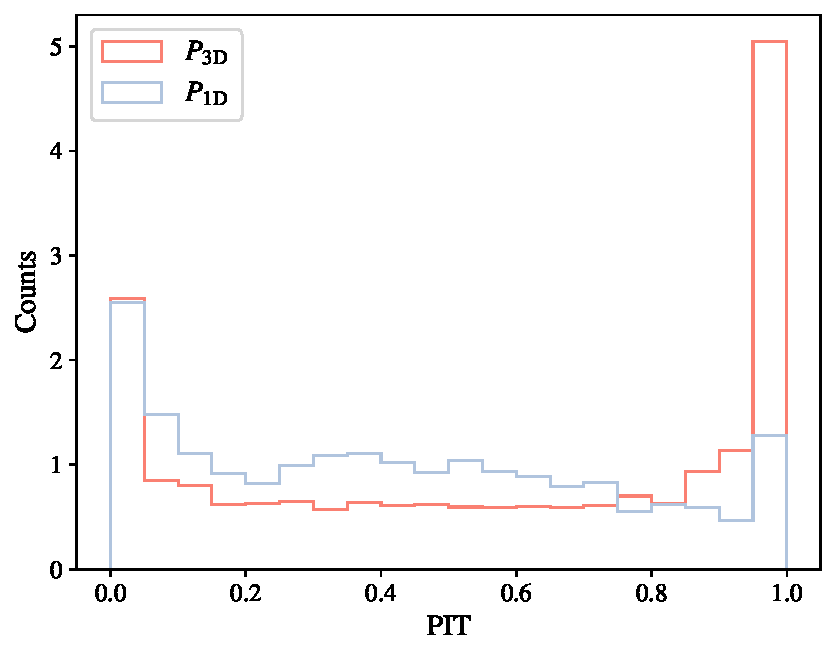
\includegraphics[width=\columnwidth]{figures/PIT_P3D.pdf}
    \caption{PIT distribution for \poned (blue) and \pthreed (red). This plot validates the uncertainties predicted by \forestflow across \lacehc simulations via a leave-simulation-out approach. The PIT distribution is approximately uniform, indicating well-calibrated uncertainties for most samples, while the peaks at the edges indicate underestimated uncertainties for some samples.}
    \label{fig:PIT}
\end{figure}
%%%%%%%%%%%%%%%%%%%

Normalizing flows predict the full posterior distribution of the target data rather than only their mean like fully-connected neural networks or their mean and width like Mixture Density Networks \citep[see][for some applications in cosmology]{ramachandra2022MachineLearningSynthetic, cabayol-garcia2023NeuralNetworkEmulator}. This is achieved through multiple sampling iterations from the target latent distribution, an 8-dimensional Gaussian in our case. In \forestflow, each sampled realization of the \pthreed model parameters is propagated to generate predictions for \pthreed and \poned (see \S\ref{sec:forestflow_NF}), producing a covariance matrix for these statistics. In this appendix, we validate its diagonal elements. Note that well-calibrated uncertainties are critical for future uses of the emulator such as cosmology inference.

We validate the uncertainty in \pthreed and \poned predictions using the Probability Integral Transform test (PIT), which is the value of the cumulative distribution function (CDF) of a distribution evaluated at the ground-truth value $z_{\rm t}$
%
\begin{equation}
    \rm{PIT} = \mathrm{CDF}[p,\,z_{\rm t}]=\int_{-\infty}^{z_{\rm t}} p(z) \mathrm{d}z\, ,
    \label{eq:pit} 
\end{equation} 
%
where $p$ is in our case the distribution of \forestflow predictions for \pthreed or \poned and $z_{\rm t}$ stands for measurements of these statistics from the simulations. A model that displays a well-calibrated uncertainty distribution yields PIT values that are uniformly distributed between zero and one. This indicates that the observed outcomes have an equal likelihood of falling at any point along the predicted CDF. In contrast, an excess of values close to zero or one indicates that the width of the distribution is underestimated.

In Fig.~\ref{fig:PIT}, we display a PIT test produced using all the \lacehc simulations via a leave-simulation-out approach (see \S\ref{sec:results_statistics}). This process validates average predictions and uncertainties against simulations excluded in the training process. The red and blue lines display the results for \pthreed and \poned, respectively, which were generated by combining results from different scales and redshifts. As we can see, the PIT distribution is approximately uniform for both statistics but it presents peaks at the low and high ends, indicating underestimated uncertainties for some samples. The cause behind this feature is unclear and it demands further investigation beyond the scope of this project.

\end{appendix}
\end{document}


